\documentclass[%twoside,                   % Impressão em frente e verso
    	        oneside,                   % Impressão apenas frente
]{configuracoes/utfpr-abntex2}
% REFERÊNCIAS------------------------------------------------------------------
\usepackage[%
    alf,
    abnt-emphasize=bf,
    bibjustif,
    recuo=0cm,
    abnt-url-package=url,       % Utiliza o pacote url
    abnt-refinfo=yes,           % Utiliza o estilo bibliográfico abnt-refinfo
    abnt-etal-cite=3,
    abnt-etal-list=3,
    abnt-thesis-year=final
]{abntex2cite}                  % Configura as citações bibliográficas conforme a norma ABNT

% PACOTES----------------------------------------------------------------------
\usepackage{subcaption}
% Utilização de figuras compostas
\usepackage[flushleft]{threeparttable}
% Utilização em tabelas
\usepackage[utf8]{inputenc}                                 % Codificação do documento
\usepackage[T1]{fontenc}                                    % Seleção de código de fonte
\usepackage{booktabs}                                       % Réguas horizontais em tabelas
\usepackage{color, colortbl}                                % Controle das cores
\usepackage{multicol}
       % Necessário para poder inserir equações lado a lado
\usepackage{float}                                          % Necessário para tabelas/figuras em ambiente multi-colunas
\usepackage{graphicx}                                       % Inclusão de gráficos e figuras
\usepackage{icomma}                                         % Uso de vírgulas em expressões matemáticas
\usepackage{indentfirst}                                    % Indenta o primeiro parágrafo de cada seção
\usepackage{microtype}                                      % Melhora a justificação do documento
\usepackage{multirow, array}                                % Permite tabelas com múltiplas linhas e colunas
\usepackage{subeqnarray}                                    % Permite subnumeração de equações
\usepackage{lastpage}                                       % Para encontrar última página do documento
\usepackage{verbatim}                                       % Permite apresentar texto tal como escrito no documento, ainda que sejam comandos Latex
\usepackage{amsfonts, amssymb, amsmath}                     % Fontes e símbolos matemáticos
\usepackage[algoruled, portuguese]{algorithm2e}             % Permite escrever algoritmos em português
%\usepackage[scaled]{helvet}                                % Usa a fonte Helvetica
\usepackage{times}                                          % Usa a fonte Times
%\usepackage{palatino}                                      % Usa a fonte Palatino
%\usepackage{lmodern}                                       % Usa a fonte Latin Modern
\usepackage[bottom]{footmisc}                               % Mantém as notas de rodapé sempre na mesma posição
\usepackage{ae, aecompl}                                    % Fontes de alta qualidade
\usepackage{latexsym}                                       % Símbolos matemáticos
\usepackage{lscape}                                         % Permite páginas em modo "paisagem"
%\usepackage{picinpar}                                      % Dispor imagens em parágrafos
%\usepackage{scalefnt}                                      % Permite redimensionar tamanho da fonte
%\usepackage{subfig}                                        % Posicionamento de figuras
%\usepackage{upgreek}                                       % Fonte letras gregas

% Redefine a fonte para uma fonte similar a Arial (fonte Helvetica)
\renewcommand*\familydefault{\sfdefault}

% CONFIGURAÇÕES DE APARÊNCIA DO PDF FINAL--------------------------------------
\makeatletter
\hypersetup{%
    portuguese,
    colorlinks=true,   % true: "links" coloridos; false: "links" em caixas de texto
    linkcolor=blue,    % Define cor dos "links" internos
    citecolor=blue,    % Define cor dos "links" para as referências bibliográficas
    filecolor=blue,    % Define cor dos "links" para arquivos
    urlcolor=blue,     % Define a cor dos "hiperlinks"
    breaklinks=true,
    pdftitle={\@title},
    pdfauthor={\@author},
    pdfkeywords={abnt, latex, abntex, abntex2}
}
\makeatother

% ALTERA O ASPECTO DA COR AZUL--------------------------------------------------
\definecolor{blue}{RGB}{41,5,195}

% REDEFINIÇÃO DE LABELS---------------------------------------------------------
\renewcommand{\algorithmautorefname}{Algoritmo}
\def\equationautorefname~#1\null{Equa\c c\~ao~(#1)\null}

% CRIA ÍNDICE REMISSIVO---------------------------------------------------------
\makeindex

% HIFENIZAÇÃO DE PALAVRAS QUE NÃO ESTÃO NO DICIONÁRIO---------------------------
\hyphenation{%
    qua-dros-cha-ve
    Kat-sa-gge-los
}

% CAPA---------------------------------------------------------------------------------------------------

% ORIENTAÇÕES GERAIS-------------------------------------------------------------------------------------
% Caso algum dos campos não se aplique ao seu trabalho, como por exemplo,
% se não houve coorientador, apenas deixe vazio.
% Exemplos: 
% \coorientador{}
% \departamento{}

% DADOS DO TRABALHO--------------------------------------------------------------------------------------
%\titulo{Título do Trabalho: Subtítulo do Trabalho}
\titulo{Reconstrução em 3D de Superfícies em Ambientes Subáquaticos Através de Dados Obtidos com Sonar MSIS}
\titleabstract{3D Surfaces Reconstruct in Underwater Environments Using Obtained Data From MSIS Sonar}
\autor{Bruno Henrique Justo da Silva}
\autorcitacao{JUSTO, Bruno} % Sobrenome em maiúsculo
\local{Rio Grande}
\data{2018}

% NATUREZA DO TRABALHO-----------------------------------------------------------------------------------
% Opções: 
% - Trabalho de Conclusão de Curso (se for Graduação)
% - Dissertação (se for Mestrado)
% - Tese (se for Doutorado)
% - Projeto de Qualificação (se for Mestrado ou Doutorado)
\projeto{Trabalho de Conclusão de Curso}

% TÍTULO ACADÊMICO---------------------------------------------------------------------------------------
% Opções:
% - Bacharel ou Tecnólogo (Se a natureza for Trabalho de Conclusão de Curso)
% - Mestre (Se a natureza for Dissertação)
% - Doutor (Se a natureza for Tese)
% - Mestre ou Doutor (Se a natureza for Projeto de Qualificação)
\tituloAcademico{Bacharel}

% ÁREA DE CONCENTRAÇÃO E LINHA DE PESQUISA---------------------------------------------------------------
% Se a natureza for Trabalho de Conclusão de Curso, deixe ambos os campos vazios
% Se for programa de Pós-graduação, indique a área de concentração e a linha de pesquisa
\areaconcentracao{}
\linhapesquisa{}

% DADOS DA INSTITUIÇÃO-----------------------------------------------------------------------------------
% Se a natureza for Trabalho de Conclusão de Curso, coloque o nome do curso de graduação em "programa"
% Formato para o logo da Instituição: \logoinstituicao{<escala>}{<caminho/nome do arquivo>}
\instituicao{Universidade Federal do Rio Grande}
\departamento{Centro de Ciências Computacionais}
\programa{Curso de Engenharia de Computação}
\logoinstituicao{0.2}{dados/figuras/logo-instituicao.png} 

% DADOS DOS ORIENTADORES---------------------------------------------------------------------------------
\orientador{Dr. Paulo Lilles Jorge Drews Junior}
%\orientador[Orientadora:]{Nome da orientadora}
\instOrientador{Centro de Ciências Computacionais -- C3}

\coorientador{Dr. Jorge Arigony Neto}
%\coorientador[Coorientadora:]{Nome da coorientadora}
\instCoorientador{Instituto de Oceanografia -- IO}

% FOLHA DE ROSTO--------------------------------------------------------------------------------------------------------

% TRABALHO DE CONCLUSÃO DE CURSO
 \preambulo{{\imprimirprojeto} apresentado ao {\imprimirprograma} da {\imprimirinstituicao}, como requisito parcial para a obtenção do título de {\imprimirtituloAcademico}.}

% DISSERTAÇÃO DE MESTRADO
% \preambulo{{\imprimirprojeto} apresentada ao Programa de \mbox{Pós-graduação} da {\imprimirinstituicao}, como requisito parcial para obtenção do título de {\imprimirtituloAcademico}.}

% TESE DE DOUTORADO
% \preambulo{{\imprimirprojeto} apresentada ao Programa de \mbox{Pós-graduação} da {\imprimirinstituicao}, como requisito parcial para a obtenção do título de {\imprimirtituloAcademico}.}

% PROJETO DE QUALIFICAÇÃO DE MESTRADO OU DOUTORADO
%\preambulo{{\imprimirprojeto} apresentado ao Programa de \mbox{Pós-graduação} da {\imprimirinstituicao}, como requisito parcial para a obtenção do título de {\imprimirtituloAcademico}.}

% OBSERVAÇÕES-----------------------------------------------------------------------------------------------------------
% Altere este arquivo APENAS comentando as linhas que não se aplicam ao tipo de trabalho acadêmico desejado.


\begin{document}

\pretextual
\imprimircapa                                               	           % Comando para imprimir Capa
\imprimirfolhaderosto{}                                     		   % Comando para imprimir Folha de rosto
% INSERE ELEMENTOS PRÉ-TEXTUAIS
% DEDICATÓRIA------------------------------------------------------------------
\renewcommand{\dedicatorianame}{DEDICATÓRIA}

\begin{dedicatoria}

Altere este texto inserindo a dedicatória do seu trabalho. 

\end{dedicatoria}
          			   % Dedicatória
% AGRADECIMENTOS---------------------------------------------------------------

\begin{agradecimentos}[AGRADECIMENTOS]

Edite e coloque aqui os agradecimentos às pessoas e/ou instituições que contribuíram para a realização do trabalho.

É obrigatório o agradecimento às instituições de fomento à pesquisa que financiaram total ou parcialmente o trabalho, inclusive no que diz respeito à concessão de bolsas.

\end{agradecimentos}
        			   % Agradecimentos
% EPÍGRAFE---------------------------------------------------------------------

\renewcommand{\epigraphname}{EPÍGRAFE}

\begin{epigrafe}

\textit{Eu denomino meu campo de Gestão do Conhecimento, mas você não pode gerenciar conhecimento. Ninguém pode. O que pode fazer - o que a empresa pode fazer - é gerenciar o ambiente que otimize o conhecimento. (PRUSAK, Laurence, 1997).}

\end{epigrafe}

% OBSERVAÇÕES------------------------------------------------------------------
% Altere o texto para inserir a epígrafe do seu trabalho
              			   % Epígrafe
% RESUMO--------------------------------------------------------------------------------

\begin{resumo}[RESUMO]
\begin{SingleSpacing}

% Não altere esta seção do texto--------------------------------------------------------
\imprimirautorcitacao. \imprimirtitulo. \imprimirdata. \pageref {LastPage} f. \imprimirprojeto\ – \imprimirprograma, \imprimirinstituicao. \imprimirlocal, \imprimirdata.\\
%---------------------------------------------------------------------------------------

O aquecimento global é o processo de aumento da temperatura média da superfície terrestre e dos oceanos causado por uma grande quantidade de gases originados de atividades humanas e emitidos na atmosfera terrestre. Um dos problemas ocasionado pelo aumento da temperatura é a diminuição da área de geleiras. Devido a importância econômica, ao seu papel como indicador de mudança no clima, além de ser o maior reservatório de água doce sobre a Terra, o monitoramento das geleiras se torna necessário e indispensável para o planeta. Esse trabalho propõe uma metodologia através do uso de algoritmos para estimar variações espaciais de superfícies submersas através da  reconstrução em 3D de superfícies a partir de dados coletados com sensor sonar MSIS. O trabalho servirá como base para ser aplicado nas superfícies submersas de geleiras com o propósito de obter uma melhor mensuração da ablação dessas superfícies.



\vspace{2em}
\textbf{Palavras-chave}: Robótica Subaquática. Reconstrução 3D. \textit{Point Cloud}, Sonar MSIS.

\end{SingleSpacing}
\end{resumo}

% OBSERVAÇÕES---------------------------------------------------------------------------
% Altere o texto inserindo o Resumo do seu trabalho.
% Escolha de 3 a 5 palavras ou termos que descrevam bem o seu trabalho 
             			   % Resumo em Português
% ABSTRACT--------------------------------------------------------------------------------

\begin{resumo}[ABSTRACT]
\begin{SingleSpacing}

% Não altere esta seção do texto--------------------------------------------------------
\imprimirautorcitacao. \imprimirtitleabstract. \imprimirdata. \pageref {LastPage} f. \imprimirprojeto\ – \imprimirprograma, \imprimirinstituicao. \imprimirlocal, \imprimirdata.\\
%---------------------------------------------------------------------------------------

%Elemento obrigatório em tese, dissertação, monografia e TCC. É a versão do resumo em português para o idioma de divulgação internacional. Deve ser antecedido pela referência do estudo. Deve aparecer em folha distinta do resumo em língua portuguesa e seguido das palavras representativas do conteúdo do estudo, isto é, das palavras-chave. Sugere-se a elaboração do resumo (Abstract) e das palavras-chave (Keywords) em inglês; para resumos em outras línguas, que não o inglês, consultar o departamento / curso de origem.\\

Acoustic images are great sources of data that can be explored in different ways for various purposes.
One of its purposes is the 3D reconstruction with data coming from images of this type, which is a branch of science understudied in the world due to the restricted application and the high cost of the equipment.
However, the area has a great potential since, through it, it is possible to reconstruct submerged environments and places, which are underexplored and practically inaccessible to humans.
Moreover, several works can be performed with reconstruction, such as volume and surface estimation in a given submerged environment or location.

The work proposes to use a methodology through the aid of algorithms to estimate spatial variations of submerged surfaces through 3D reconstruction, from data collected with MSIS (Mechanical Scanning Image Sonar) sonar sensor.
The objective of using the MSIS model is to cost reduce, since the risk of loss of equipment is high in places where there is low contact with the operator.
The work may serve as a base to be applied to the glaciers submerged surfaces in order to obtain a better measurement of the ablation of then.

\vspace{2em}
\textbf{Keywords}: Underwater Robotics. 3D Reconstruction. Point Cloud. Sonar MSIS.

\end{SingleSpacing}
\end{resumo}

% OBSERVAÇÕES---------------------------------------------------------------------------
% Altere o texto inserindo o Abstract do seu trabalho.
% Escolha de 3 a 5 palavras ou termos que descrevam bem o seu trabalho 
             		           % Resumo em Inglês
% Lista de Figuras----------------------------------------------------------------

\pdfbookmark[0]{\listfigurename}{lof}
\listoffigures*
\cleardoublepage

% OBSERVAÇÕES---------------------------------------------------------------------
% Este arquivo não precisa de ser alterado, pois a lista é gerada automaticamente.
   % Lista de Figuras
%% LISTA DE QUADROS----------------------------------------------------------------

\renewcommand{\listofquadrosname}{LISTA DE QUADROS}

\pdfbookmark[0]{\listofquadrosname}{loq}
\listofquadros*
\cleardoublepage

% OBSERVAÇÕES---------------------------------------------------------------------
% Este arquivo não necessita de ser editado. A lista é gerada automaticamente.
   % Lista de Quadros
% LISTA DE TABELAS-------------------------------------------------------------

\pdfbookmark[0]{\listtablename}{lot}
\listoftables*
\cleardoublepage

% OBSERVAÇÕES-------------------------------------------------------------------
% Este arquivo não precisa ser alterado, pois a lista é gerada automaticamente.
         		   % Lista de Tabelas
% LISTA DE ABREVIATURAS E SIGLAS----------------------------------------------------------

\begin{siglas}
    \item[C3] Centro de Ciências Computacionais
    \item[CPU] Unidade Central de Processamento, do inglês \textit{Central Process Unit}
    \item[FLS] Sonar de Imageamento Frontal, do inglês \textit{Forwarding Look Sonar}.
    \item[FURG] Universidade Federal do Rio Grande
    \item[GPU] Unidade de Processamento Gráfico, do inglês \textit{Graphics Processing Unit}
    \item[LACRIO] Laboratório de Monitoramento da Criosfera
    \item[MSIS] do inglês \textit{Mechanical Scanning Image Sonar}
    \item[MLS] do inglês \textit{Moving Least Squares}
    \item[NAUTEC] Grupo de Pesquisa em Automação e Robótica Inteligente
    \item[OSG] do inglês \textit{Open Scene Graph}
    \item[P2P] do inglês \textit{Peer-to-Peer}
    \item[PCL] Biblioteca de Nuvem de Pontos, do inglês \textit{Point Cloud Library}
    \item[ROCK] do inglês \textit{Robot Construction Kit}
    \item[ROS] Sistema Operacional de Robôs, do inglês \textit{Robot Operating System}
    \item[ROV] Robô Operado Remotamente, do inglês \textit{Remotely Operated Vehicle}
    \item[SONAR] Navegação e Determinação da Distância pelo Som, do inglês \textit{Sound Navigation and Ranging}
    \item[SORF] Filtro Estatístico de Remoção de \textit{Outliers}, do inglês \textit{Statistical Outlier Removal Filter}
    \item[UUV] Veículo Submarino Não Tripulado, do inglês \textit{Unmanned Underwater Vehicle}
\end{siglas}



% OBSERVAÇÕES-----------------------------------------------------------------------------
% Altere a lista acima para definir os acrônimos e siglas utilizados neste trabalho
          		   % Lista de Abreviaturas e Siglas
%% LISTA DE SÍMBOLOS------------------------------------------------------------

\begin{simbolos}
    \item[$ \Gamma $] Letra grega Gama
    \item[$ \lambda $] Comprimento de onda
    \item[$ \in $] Pertence
\end{simbolos}

% OBSERVAÇÕES-------------------------------------------------------------------
% Altere a lista acima para definir os símbolos utilizados no trabalho
        		   % Lista de Símbolos
%% LISTA DE ALGORITMOS----------------------------------------------------------

\newcommand{\algoritmoname}{Algoritmo}
\renewcommand{\listalgorithmcfname}{LISTA DE ALGORITMOS}

\floatname{algocf}{\algoritmoname}
\newlistof{listofalgoritmos}{loa}{\listalgoritmoname}
\newlistentry{algocf}{loa}{0}

\counterwithout{algocf}{chapter}
\renewcommand{\cftalgocfname}{\algoritmoname\space}
\renewcommand*{\cftalgocfaftersnum}{\hfill--\hfill}

\pdfbookmark[0]{\listalgorithmcfname}{loa}
\listofalgorithms
\cleardoublepage

% OBSERVAÇÕES------------------------------------------------------------------
% Este arquivo não precisa ser alterado, pois a lista é gerada automaticamente.
   % Lista de Algoritmos
% SUMÁRIO----------------------------------------------------------------------

\renewcommand{\contentsname}{SUMÁRIO}

\pdfbookmark[0]{\contentsname}{toc}
\tableofcontents*
\cleardoublepage

% OBSERVAÇÕES-------------------------------------------------------------------
% Este arquivo não precisa ser alterado, pois o sumário é gerado automaticamente.
               			   % Sumário

\textual
% INSERE ELEMENTOS TEXTUAIS
% INTRODUÇÃO-------------------------------------------------------------------

\chapter{INTRODUÇÃO}
\label{chap:introducao}

\section{Motivação}
\label{sec:motivacao}

O aquecimento global é o processo de aumento da temperatura média da superfície terrestre e dos oceanos, causado por uma grande quantidade de gases, como o dióxido de carbono ($CO_2$) e o metano ($CH_4$), originados de atividades humanas e emitidos na atmosfera terrestre provocando grandes impactos ambientais negativos. Os principais impactos causados pelo aquecimento global são: aumento de eventos de extremo climático (ciclones, ondas de calor, chuvas torrenciais, etc), redução de biodiversidade, elevação do nível do mar e da temperatura na superfície terrestre, etc. 

A temperatura da superfície global aumentou cerca de 0.2 \textordmasculine C em três décadas e 0.8 \textordmasculine C no último século \cite{hansen2006global}. Para ilustrar esse retrato, a Figura \ref{fig:ast-and-sl}-A mostra as mudanças na temperatura média da superfície terrestre enquanto a Figura \ref{fig:ast-and-sl}-B exibe as mudanças no nível médio do mar. Essas mudanças ocorreram no intervalo de 1986 a 2005.

\begin{figure}[H]
    \centering
    \caption{(A) Mudança na temperatura média da superfície terrestre (1986 -- 2005). (B) Mudança do nível médio do mar (1986 -- 2005).}
    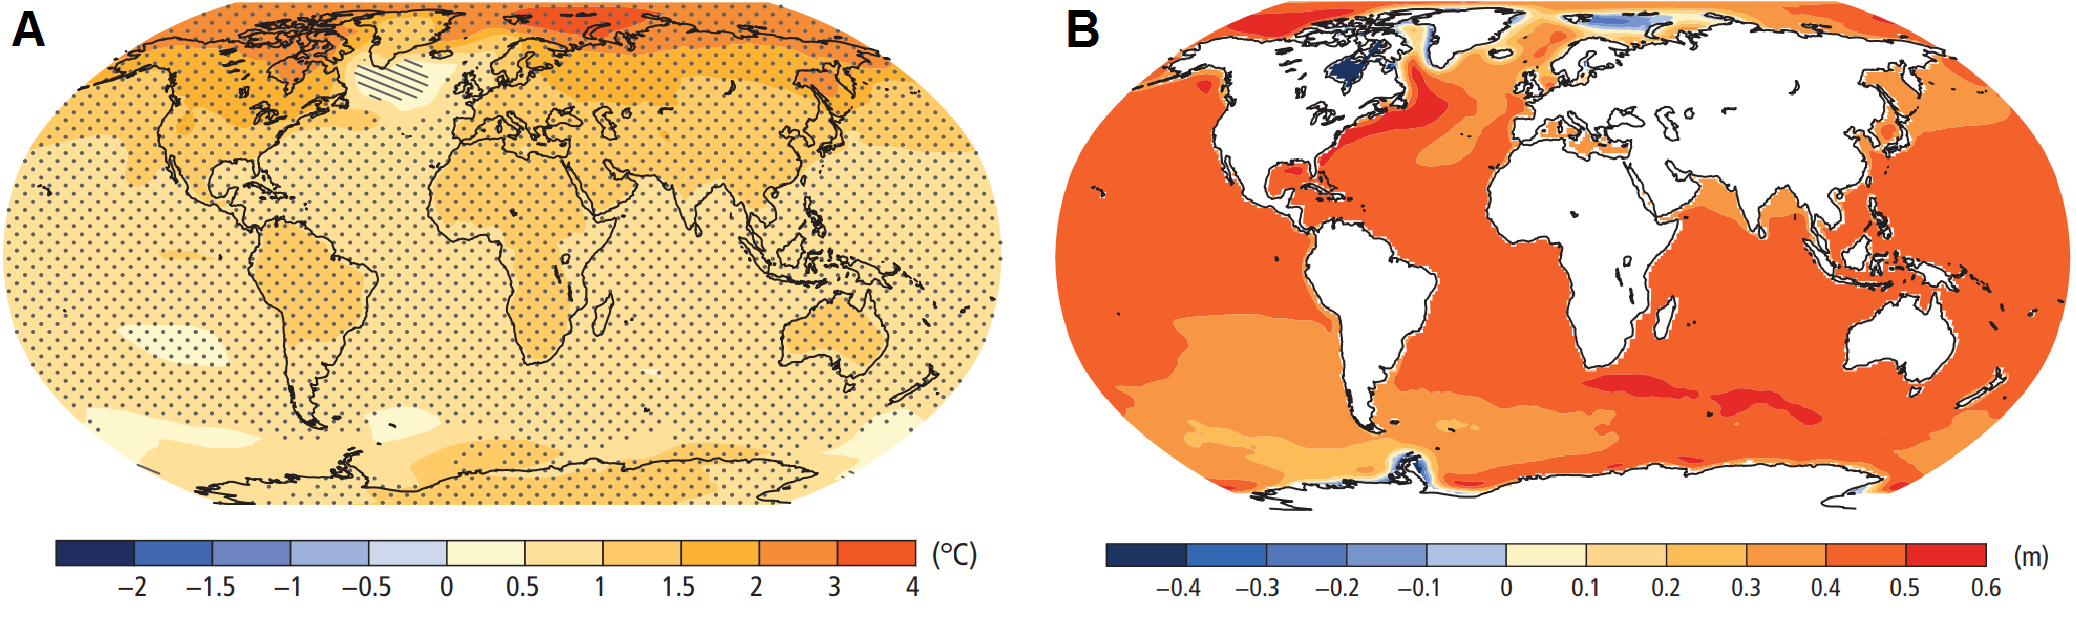
\includegraphics[scale=0.27]{dados/figuras/ast-and-sl.png}
    \fonte{Adaptado de \cite{pachauri2014climate}.}
    \label{fig:ast-and-sl}
\end{figure}

A redução da criosfera é um dos problemas ocasionado pelo aumento da temperatura e do nível do mar. A criosfera é constituída por regiões da superfície terrestre cobertas permanentemente por gelo e neve ou o solo é constituído por gelo, como por exemplo: lagos e rios congelados, mantos e calotas de gelo, neve sazonal e geleiras.

Em destaque, as geleiras do planeta estão perdendo massa, tornando uma das principais causas para o aumento no nível dos oceanos \cite{rietbroek2016revisiting}. Devido a importância econômica, ao seu papel como indicador de mudança no clima, além de ser o maior reservatório de água doce sobre a Terra, perdendo em volume total de água apenas para os oceanos \cite{pinto2015crise}, o monitoramento das geleiras se torna indispensável para o planeta.

Entretanto, a maior parte das geleiras estão em locais remotos, dificultando o acesso e a logística à essas áreas. Por consequência, os estudos com o sensoriamento remoto se tornou uma alternativa comumente utilizada para a estimação de balanço de massa. Porém, os satélites não são eficazes para coletar informações de geleiras que possuem uma parcela submersa, visto que a tecnologia do sensoriamento remoto só captura informações da superfície terrestre, impedindo coletar informações a respeito do que está entre a superfície e o fundo de corpos d'água. 
A Figura \ref{fig:remote_sensor} mostra o mecanismo de aquisição de dados do sensoriamento remoto. A obtenção de informações é realizada por meio do registro do retorno da interação da radiação eletromagnética provida do Sol com a superfície terrestre. 

\begin{figure}[H]
    \centering
    \caption{Aquisição de dados do sensoriamento remoto.}
    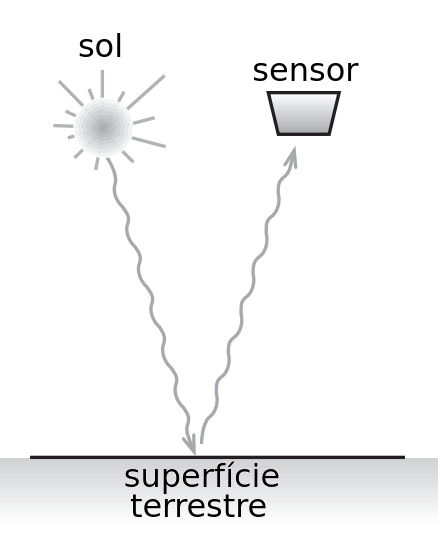
\includegraphics[scale=0.5]{dados/figuras/remote_sensor.png}
    \label{fig:remote_sensor}
    \fonte{Adaptado de \cite{kerle2004principles}.}
\end{figure}

Para coletar informações em ambientes submersos torna-se mais adequado utilizar sensores que operam com ondas sonoras, pois essas se propagam melhor em ambientes com maior densidade, como o fundo de oceanos e lagos.

\section{Objetivos}
\label{sec:objetivos}

O objetivo principal do trabalho é utilizar uma plataforma robótica do tipo ROV (Robô Operado Remotamente, do inglês \textit{Remotely Operated Vehicle}) equipada com um sensor sonar MSIS (do inglês \textit{Mechanical Scanning Image Sonar}) para estimar variações espaciais (balanço de massa) de superfícies submersas por meio da reconstrução em 3D de capturas temporalmente espaçadas de imagens acústicas. 
Para atingir o objetivo principal, será necessário alcançar tais objetivos:

\begin{itemize}
    \item Estudar o mecanismo e eficiência da aquisição de imagens do sonar MSIS e os principais métodos para manipular imagens acústicas;
    \item Coletar dados em simulação e \textit{in loco} utilizando robô subaquático acoplado com sonar e sensores auxiliares;
    \item Reconstruir as superfícies submersas utilizando algoritmos de reconstrução com o auxílio de bibliotecas de nuvem de pontos;
    \item Comparar modelos reconstruídos com o intuito de analisar a perda/ganho de volume entre eles. 
\end{itemize}
\hspace{1em}

Para a efetivação dos objetivos, o NAUTEC (Grupo de Pesquisa em Automação e Robótica Inteligente) junto ao C3 (Centro de Ciências Computacionais), disponibilizará a plataforma robótica, o sensor sonar e sensores auxiliares. Este trabalho é o inicio dos estudos para uma melhor precisão na estimação da ablação\footnote{Ablação é a perda de massa/energia de um sistema, nessa circunstância, a fusão e sublimação do gelo.} e o conhecimento de características da parte frontal submersa de geleiras, tais como configuração física e comportamento de degelo, que será uma contribuição para o LACRIO (Laboratório de Monitoramento da Criosfera). Além disso, o trabalho contribuirá para a consolidação da área da robótica subaquática na FURG (Universiade Federal do Rio Grande).

Embora o trabalho prático seja realizada em ambiente não glacial, a intenção do projeto é, posteriormente, ser executado em geleiras.

\section{Organização do Trabalho}
\label{sec:organizacaoTrabalho}

Primeiramente, após o capítulo de introdução, o Capítulo \ref{chap:fundamentacaoTeorica} apresenta assuntos fundamentais para a compreensão do mesmo, como a descrição do sensor e dos \textit{softwares} utilizados. No terceiro capítulo, é abordado detalhadamente a metodologia utilizada e seus motivos. O Capítulo \ref{chap:resultados} apresenta os resultados que foram obtidos no experimento. 
%Por último, o capítulo \ref{chap:conclusao} encerra o trabalho com a opinião do autor sobre o desenvolvimento e resultados obtidos.                		                % Introdução
\chapter{FUNDAMENTAÇÃO TEÓRICA}
\label{chap:fundamentacaoTeorica}

% FUNDAMENTAÇÃO-TEÓRICA-------------------------------------------------------

\section{Sensor Sonar}
\label{sec:sonar}

\subsection{Princípio do Sonar}
\label{sec:principio-sonar}

O sonar é um sensor capaz de calcular a distância de objetos em um meio através de ondas sonoras. O sensor emite um pulso de onda que percorre o meio até colidir em um obstáculo/objeto ou ser absorvido completamente pelo meio. Após colidir, parte da onda é refletida e retorna para o sensor (a origem do pulso) com uma intensidade menor. Ao ser captada pelo sensor, a onda é decomposta em várias partes, onde cada parte é conhecida como \textit{bin}. O conjunto de \textit{bins} que compõe uma onda, é chamado de \textit{beam}, como mostra a Figura \ref{fig:imagem_acustica}.

De maneira geral, o sonar poder ser do tipo passivo ou ativo. O sonar passivo apenas escuta o meio com o intuito de filtrar os sinais sonoros de diferentes objetos do ruído do ambiente. Ao passo que, o sonar ativo tem a capacidade de emitir sinais acústicos e captar o retorno do pulso. O alcance de um pulso de um sonar ativo e a qualidade do sinal\footnote{Quanto maior a qualidade do sinal, maior será o nível de detalhamento e discriminação do alvo e menor será a quantidade de ruído.} retornado está relacionado com a frequência de operação do sensor (Tabela \ref{tab:freq-acustica}).

\begin{figure}[H]
    \centering
    \caption{Representação de um \textit{bin} e um \textit{beam} em uma imagem acústica}
    \label{fig:imagem_acustica}
    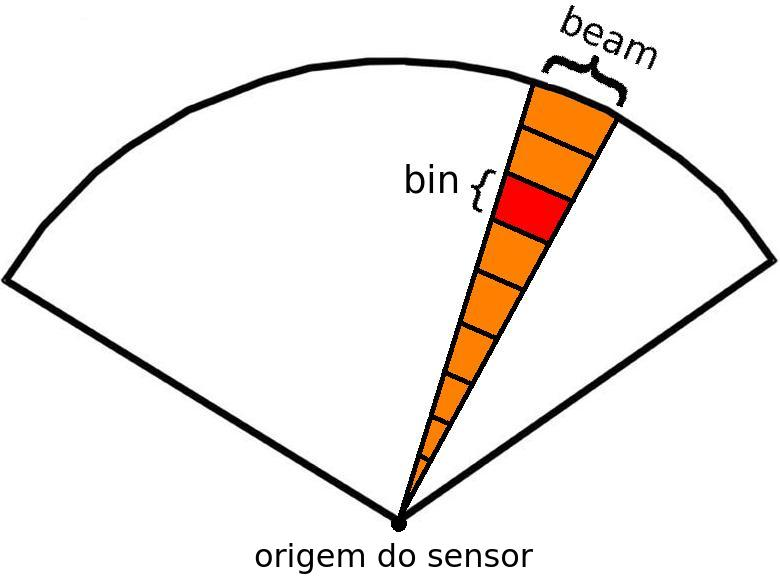
\includegraphics[scale=0.3]{dados/figuras/imagem_acustica.jpg}
\end{figure}

Sinais de alta frequência possuem um curto alcance, porém produz um sinal de retorno que carrega mais informações e com uma alta qualidade. Ao contrário, os sinais de baixa frequência são menos atenuados pelo meio, resultando em uma melhor propagação, mas em compensação, a quantidade de informação no sinal de retorno é menor.

\begin{table}[H]
    \centering
    \caption{Relação entre alcance e frequência da onda acústica}
    \label{tab:freq-acustica}
    \begin{tabular}{@{}lll@{}}
    \toprule
        Frequência & Tamanho da onda & Alcance \\ \midrule
        100 Hz & 15 m & 1000 km ou mais \\
        1 kHz & 1.5 m & 100 km ou mais \\
        10 kHz & 15 cm & 10 km \\
        25 kHz & 6 cm & 3 km \\
        50 kHz & 3 cm & 1 km \\
        100 kHz & 1.5 cm & 600 m \\
        500 kHz & 3 mm & 150 m \\
        1 MHz & 1.5 mm & 50 m \\ \bottomrule
    \end{tabular}
    \fonte{\cite{christ2013rov}}
\end{table}

Sabendo a velocidade de propagação do som no meio e o intervalo de tempo que a onda levou para retornar, é possível calcular a distância do obstáculo até o sensor. 
Definimos como \textit{ping} a ída e retorno de um pulso de som emitido pelo sensor, e tempo de \textit{ping} como o intervalo de tempo para realizar um \textit{ping}. 
A velocidade de propagação do som é maior nos sólidos, pois as moléculas estão mais próximas, transmitindo a energia cinética da onda de umas para as outras com maior facilidade. 
Na Tabela \ref{tab:vel_som}, \cite{halliday2008fundamentals} comprovou esse fato, onde se encontra diferentes velocidades do som de acordo com o meio.

\begin{table}[H]
    \centering
    \begin{threeparttable}
    \caption{Velocidade do som em diferentes meios.}
    \label{tab:vel_som}
    \begin{tabular}{lc}
        \toprule
            \textbf{Meio$^a$} & \textbf{Velocidade (m/s)} \\ 
        \midrule
            \textit{Gases} &  \\
            Ar (0 º C) & 331 \\
            Ar (20 º C) & 343 \\
            Hélio & 965 \\
            Hidrogênio & 1284 \\
            \textit{Líquidos} &  \\
            Água (0 º C) & 1402 \\
            Água (20 º C) & 1482 \\
            Água salgada$^b$ & 1522 \\
            \textit{Sólidos} &  \\
            Aço & 5941 \\
            Alumínio & 6420 \\
            Granito & 6000 \\ \bottomrule
    \end{tabular}
    \begin{tablenotes}
        \item $^a$ A 0 º C e 1 atm de presssão, a menos que haja uma indicação em contrário.
        \item $^b$ A 20 º C e 3,5\% de salinidade.
    \end{tablenotes}
    \end{threeparttable}
    \fonte{\cite{halliday2008fundamentals}.}
\end{table}


\subsection{Sonar \textit{Singlebeam} e \textit{Multibeam}}
\label{sec:single-multibeam}
Além da classificação passiva e ativa, o sonar pode ser agrupado de diversas maneiras, uma delas referente a área de cobertura do sinal.
O sonar \textit{singlebeam} trabalha com apenas um único pulso de onda (Figura \ref{fig:echo-sounder}). Geralmente ele é encontrado na parte inferior dos robôs e posicionado para baixo com o objetivo de encontrar a altitude do robô em relação ao fundo do corpo d'água em que está. Ainda pode ser posicionado nas partes laterais, frontal ou posterior para ser utilizado como um sensor de colisão.

\begin{figure}[H]
    \centering
    \caption{Diferentes modelos de sonares.}
    \label{fig:beams}
    \begin{subfigure}[t]{0.4\textwidth}
        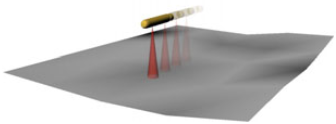
\includegraphics[width=\textwidth]{dados/figuras/singlebeam.png}
        \caption{\textit{Echo sounder.}}
        \label{fig:echo-sounder}
    \end{subfigure}
    \begin{subfigure}[t]{0.4\textwidth}
        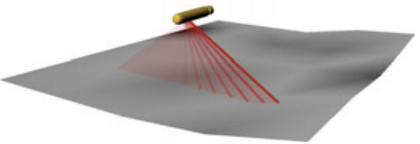
\includegraphics[width=\textwidth]{dados/figuras/mec-scan-profiling.png}
        \caption{\textit{Mechanically scanned profiler.}}
        \label{fig:mec-scan-prof}
    \end{subfigure}
    \begin{subfigure}[t]{0.4\textwidth}
        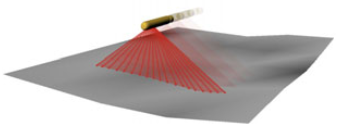
\includegraphics[width=\textwidth]{dados/figuras/multibeam.png}
        \caption{\textit{Multibeam echo sounder.}}
        \label{fig:multi-prof-sonar}
    \end{subfigure}
    \begin{subfigure}[t]{0.4\textwidth}
        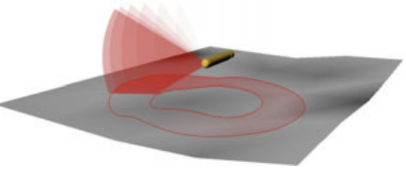
\includegraphics[width=\textwidth]{dados/figuras/msis.png}
        \caption{\textit{Mechanical scanning imaging sonar.}}
        \label{fig:msis}
    \end{subfigure}
    \begin{subfigure}[t]{0.4\textwidth}
        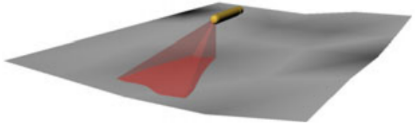
\includegraphics[width=\textwidth]{dados/figuras/fls.png}
        \caption{\textit{Foward looking imaging sonar.}}
        \label{fig:fls}
    \end{subfigure}
    \fonte{Adaptado de \cite{ribas2010underwater}.}
\end{figure}

Por outro lado, o sonar \textit{multibeam} é mais complexo, composto por um conjunto de hidrofones\footnote{Os hidrofones são transdutores de som para eletricidade que captam vibrações sonoras transmitidas no meio, reconhecendo na forma de frequência. Após reconhecer a frequência, o dispositivo transforma em um sinal elétrico.} que emitem vários pulsos de onda de forma simultânea, que juntos possuem o formato de um leque (Figuras \ref{fig:multi-prof-sonar} e \ref{fig:fls}). Esse tipo de sonar é comumente utilizado para fazer batimetria e imageamento de ambientes e superfícies submersas por possuir uma alta qualidade e velocidade de coleta de dados.

\subsection{Sonar MSIS}
\label{sec:msis}
O MSIS (do inglês \textit{Mechanical Scanning Image Sonar}) é um sonar mecânico \textit{singlebeam} de varredura de 360º, ou seja, possui um atuador no cabeçote do sensor para poder girar a partir de passos pré-definidos e imagear o ambiente em seu entorno, ilustrado na Figura \ref{fig:msis}. 
O sensor realiza o escaneamento no plano horizontal, onde o cabeçote gira em um incremento de um ângulo pré-estabelecido, efetuando uma leitura para cada incremento, como mostra a Figura \ref{fig:msis-scanning}.
Para exemplificar, na Figura \ref{fig:msis-image}, apresenta uma imagem de satélite de uma doca com a sobreposição de uma imagem acústica obtida com um MSIS.

\begin{figure}[H]
    \centering
    \caption{Imagem acústica sobreposta em uma imagem de satélite.}
    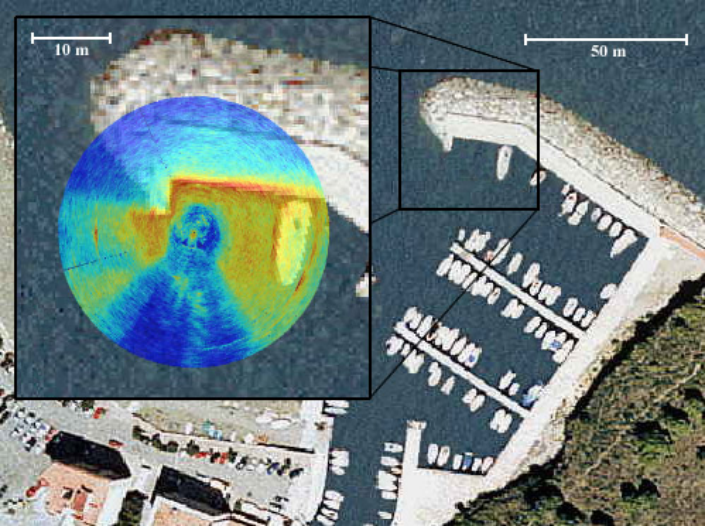
\includegraphics[scale=0.3]{dados/figuras/msis_image.png}
    \fonte{\cite{ribas2006slam}}
    \label{fig:msis-image}
\end{figure}

\begin{figure}[H]
    \centering
    \caption{Representação do processo de escaneamento de um MSIS.}
    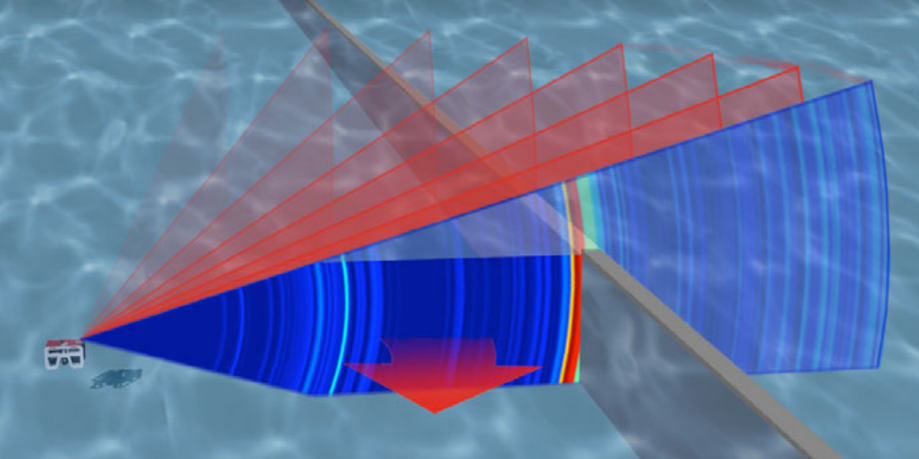
\includegraphics[scale=0.3]{dados/figuras/msis-scanning.png}
    \fonte{\cite{ribas2010underwater}}
    \label{fig:msis-scanning}
\end{figure}

O processo de escaneamento pode ser vagaroso por conta do transdutor rotar os 360 graus\footnote{Geralmente o equipamento possibilita a configuração para um range angular menor do que 360º, tornando menor o tempo de leitura de uma imagem completa.}, porém seu baixo custo e peso torna o modelo viável para aplicações com alto risco de perda do equipamento como no caso das geleiras.

%Precisa falar dos problemas com o MSIS (shadows, imagens distorcidas, ambiguidades, etc..)

\section{\textit{Robot Operating System}}
\label{sec:ros}

O ROS (Sistema Operacional de Robôs, do inglês \textit{Robot Operating System}) é uma plataforma de desenvolvimento de softwares (\textit{framework}) de código aberto direcionado para a área da robótica, que fornece a funcionalidade de um meta-sistema operacional, tais como, abstração de hardware, gerenciamento de pacotes, controle de dispositivos de baixo nível e troca de mensagens entre processos. 
O ROS atua como um \textit{middleware} de comunicação entre aplicações robóticas e o \textit{hardware}, oferecendo ferramentas e bibliotecas para auxiliar no desenvolvimento e execução de aplicações robóticas distribuídas. Os conjuntos de processos em execução do ROS são representados através de uma arquitetura de grafos orientados ou grafos de computação.

\subsection{Grafos de computação}

No ROS, os grafos de computação possui a finalidade de representar sua rede de comunicação P2P entre os processos. O grafo computacional é composto pelos seguintes elementos:

\begin{itemize}
    \addtolength{\itemindent}{2em}
    \setlength\itemsep{1em}
    
    \item Nodos: Os nodos são os processos em execução no sistema e são responsáveis por realizar funções computacionais.  Em um sistema ROS pode haver vários nodos responsáveis por controlar apenas um único robô, como por exemplo, um nodo responsável por controlar a localização do robô, outro nodo controla o sensor laser, outro faz o planejamento da rota, entre outros;
    
    \item Mensagens: As mensagens são estruturas de dados que podem incluir diversos tipos de dados, como inteiros, boleanos, strings, etc. Através das trocas de mensagens, os nodos fazem a comunicação entre si;
    
    \item Tópicos: Os tópicos são canais de comunicação que adotam a semântica de publicação/inscrição de mensagens. Os nodos utilizam essa semântica para publicar mensagens e/ou se inscreverem nos tópicos. Portanto, se um nodo publicar mensagens em um determinado tópico, todos os os nodos inscritos nesse tópico receberão as mensagens. Além disso, podem haver múltiplos nodos inscritos e/ou publicando em um mesmo tópico, assim como um nodo pode publicar e se inscrever em múltiplos tópicos. A Figura \ref{fig:topic_node} ilustra a relação entre nodo e tópico;
    
    \item Serviços: Diferente dos tópicos, os serviços possibilitam uma comunicação direta entre processos, através de interações requisição/resposta que é comumente empregado em sistemas distribuídos;
    
    \item \textit{Bags}: O \textit{bag} é um formato de arquivo usado pelo ROS para gravar e reproduzir dados gerados em um procedimento. Eles são extremamente importantes, pois proporcionam ao usuário gravar dados de sensores e atuadores para poder reproduzir futuramente;
    
    \item \textit{Master}: O \textit{master} permite que os nodos localizem uns aos outros para trocar mensagens ou invocar serviços. Uma vez que os nodos se localizaram através de consultas ao \textit{master}, uma comunicação direta P2P entre os nodos é estabelecida. Além disso, ele tem a tarefa de registrar nodos, tópicos, serviços e parâmetros da rede;
    
    \item Servidor de parâmetros: O servidor de parâmetros faz parte do \textit{master}. Ele é responsável por permitir o compartilhamento distribuído de parâmetros em tempo de execução aos nodos.
\end{itemize}
\hspace{1em}

\begin{figure}[H]
    \centering
    \caption{Relação entre tópico e nodo.}
    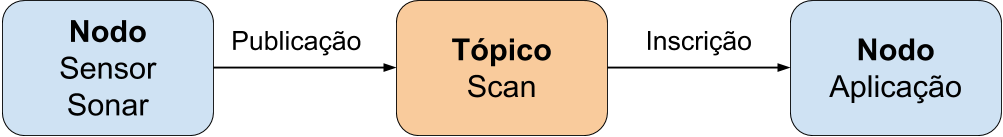
\includegraphics[scale=0.3]{dados/figuras/topic_node.png}
    \label{fig:topic_node}
\end{figure}

A Figura \ref{fig:topic_node} ilustra com um exemplo, o funcionamento da estrutura de tópicos e nodos do ROS. O nodo \textit{Sensor Sonar} é responsável por aquirir os dados da coleta e publicar esses dados no tópico \textit{Scan}. Já o nodo \textit{Aplicação} recebe os dados do tópico \textit{Scan} e com base nesses dados realiza ações, como por exemplo, evitar uma colisão do robô com objetos no ambiente.

\section{Simulador Gazebo}
\label{sec:gazebo}

O Gazebo é um robusto \textit{software} de código aberto para simulação de ambientes virtuais 3D para robôs. O simulador possui uma excelente ferramenta de simulação física, gráficos de alta qualidade, interface gráfica, ferramentas de criação de cenários realísticos e robôs, entre outras qualidades. Além disso, o \textit{software} é integrado com o ROS, colaborando para o desenvolvimento de algoritmos, componentes, dispositivos e resoluções de problemas na área da robótica. A interface gráfica é acessível e intuitiva para o usuário, permitindo manipular o ambiente e seus elementos de forma fácil, como ilustra a Figura \ref{fig:gazebo}. Porém, a simulação em ambientes submersos ainda não está próximo do real, pois a ferramenta ainda não é capaz de adicionar uma das principais características contida no meio subaquático e fundamental para o desenvolvimento da área da visão subaquática, a turbidez na água. 

\begin{figure}[H]
    \centering
    \caption{Interface gráfica do simulador Gazebo}
    \label{fig:gazebo}
    \begin{subfigure}[t]{0.45\textwidth}
        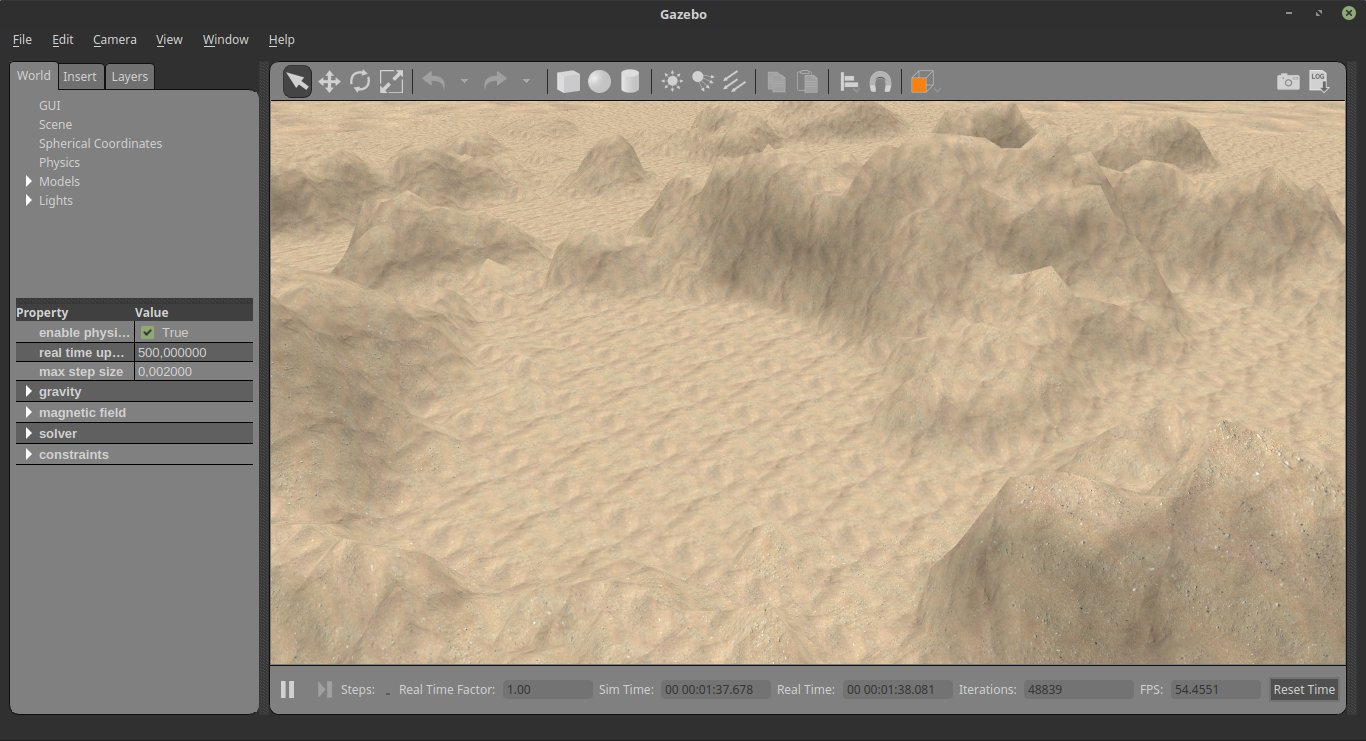
\includegraphics[width=\textwidth]{dados/figuras/gazebo1.jpeg}
    \end{subfigure}
    \begin{subfigure}[t]{0.45\textwidth}
        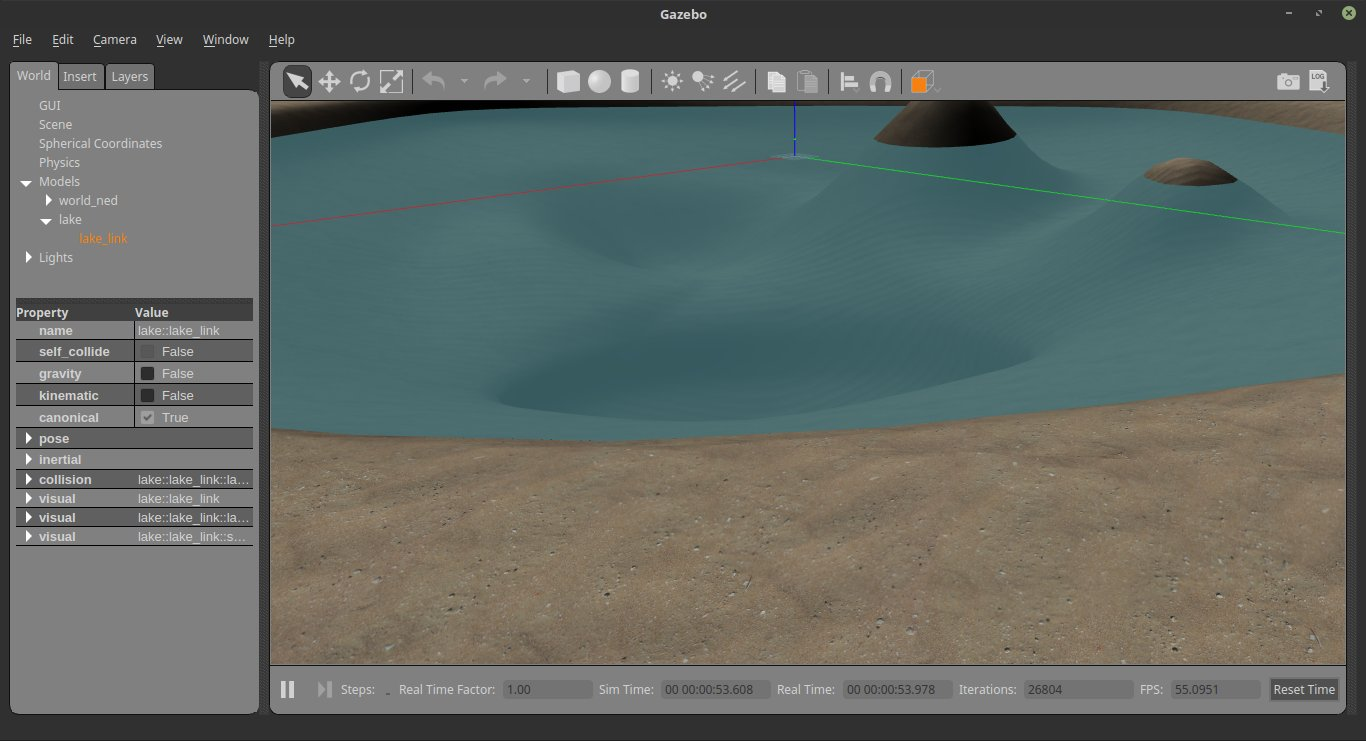
\includegraphics[width=\textwidth]{dados/figuras/gazebo2.jpeg}
    \end{subfigure}
    \begin{subfigure}[t]{0.45\textwidth}
        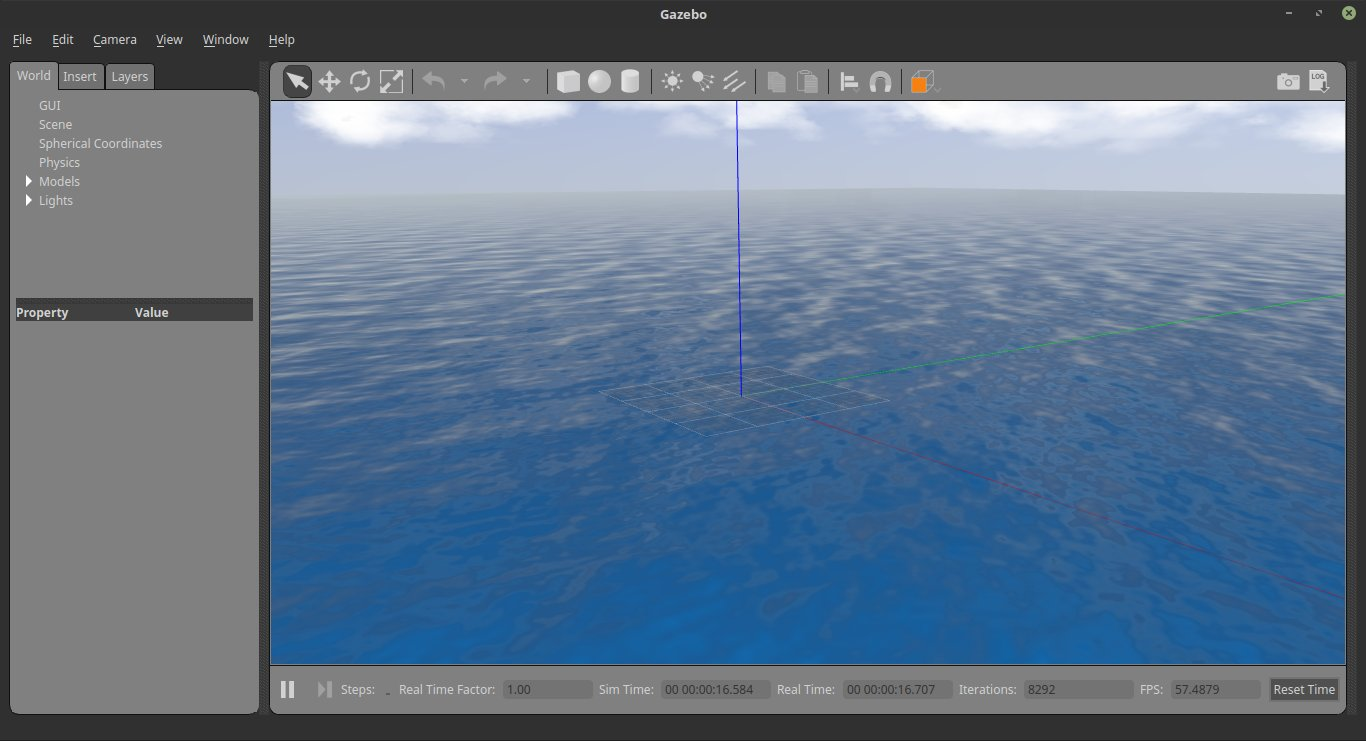
\includegraphics[width=\textwidth]{dados/figuras/gazebo3.jpeg}
    \end{subfigure}
    \begin{subfigure}[t]{0.45\textwidth}
        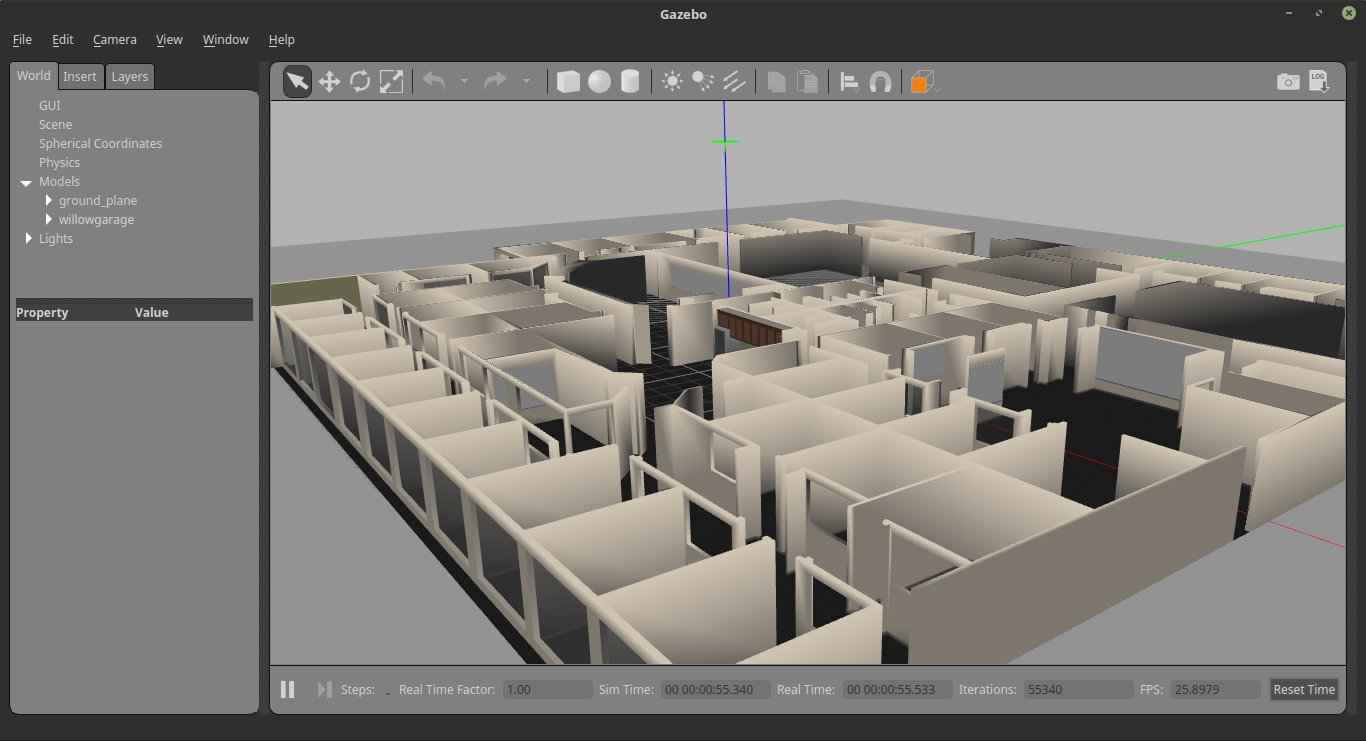
\includegraphics[width=\textwidth]{dados/figuras/gazebo4.jpeg}
    \end{subfigure}
\end{figure}

Contudo, o desenvolvimento em código aberto facilita a criação de pacotes com plugins que auxiliam na simulação, como os pacotes \textit{UUV Simulator} e o Simulador Netuno, desenvolvido por, respectivamente, \cite{manhaes2016uuv} e \cite{longaray2017}. Ambos trabalhos contribuíram para a expansão da área da robótica subaquática.

\section{\textit{GPU Sonar Simulatior}}
\label{sec:gpu_sonar_sim}

O \textit{GPU Sonar Simulator} é um simulador baseado no método proposto por \cite{cerqueira2016gpu}, que utiliza \textit{shaders} para processar imagens de sonar MSIS e FLS com baixo custo computacional. 
Os \textit{shaders} são um conjunto de instruções que definem o comportamento da superfície dos objetos em um processamento gráfico.
Eles são executados na GPU do computador, que é o processador dedicado especialmente para a renderização de gráficos em tempo real. 
Seu funcionamento é determinado pelo \textit{pixel pipeline} ou \textit{pipeline} de renderização 3D, que é a unidade encarregada pela transferência de dados referentes aos pixels que formam uma imagem. 
Portanto, o \textit{pipeline} de renderização 3D é exclusivamente processado na GPU, resultando em uma redução na utilização de recursos da CPU e acelerando o processamento gráfico do computador. 

O simulador foi inicialmente criado para a plataforma ROCK\footnote{O ROCK é um \textit{framework} para o desenvolvimento de sistemas robóticos, semelhante ao ROS. Saiba mais em: \url{https://www.rock-robotics.org/}} (do inglês \textit{Robot Construction Kit}), porém através do trabalho de \cite{longaray2017} foi realizada a adaptação para o ROS.
No desenvolvimento foi utilizado a linguagem \textit{C++} e a ferramenta OSG\footnote{O OSG é um conjunto de ferramentas gráficas 3D de alta performance de código livre e desenvolvida na linguagem \textit{C/C++}. Saiba mais em: \url{http://www.openscenegraph.org/}} (do inglês \textit{Open Scene Graph}).
Quando um ambiente é renderizado no OSG, o \textit{shader} computa dados em um processamento a partir de uma câmera inserida na cena, onde tais dados são divididos em três categorias: 

\begin{itemize}
    \item Intensidade: simula a energia acústica refletida do objeto baseado no ângulo da superfície de contato;
    \item Profundidade: retrata a distância euclidiana entre o ponto central da câmera e o ponto da superfície de contato do obstáculo;
    \item Distorção angular: representa o ângulo entre a coluna central e as colunas nas extremidades da câmera.
\end{itemize}

A intensidade é calculada de acordo com os canais azul e verde, que representam, respectivamente, a intensidade e a distância, como mostra a Figura \ref{fig:shader_output}. Quanto mais claro é o azul em um determinado ponto, maior é a intensidade da energia acústica refletida, ao passo que quanto mais claro for o verde, maior é a distância ou profundidade do sensor até o ponto.

\begin{figure}[H]
    \centering
    \caption{Imagens correspondentes geradas pelo \textit{GPU Sonar Simulator}}
    \label{fig:shader_output}
    \begin{subfigure}[t]{0.5\textwidth}
        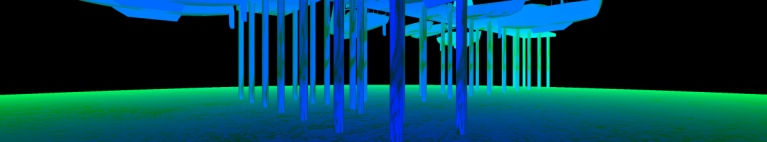
\includegraphics[width=\textwidth]{dados/figuras/shader_output1.png}
        \caption{Imagem gerada pelo \textit{shader}}
    \end{subfigure}
    \begin{subfigure}[t]{0.5\textwidth}
        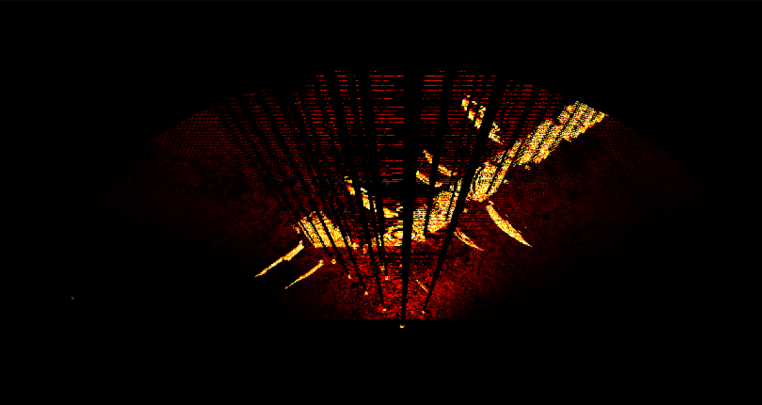
\includegraphics[width=\textwidth]{dados/figuras/shader_output2.png}
        \caption{Imagem acústica resultante.}
    \end{subfigure}
    \fonte{Adaptado de \cite{longaray2017}.}
\end{figure}

O simulador do sonar possui alguns parâmetros de simulação que são definidos pelo usuário, tais como:

\begin{itemize}
    \item Quantidade de \textit{beams}: Define o número de colunas que a imagem será dividida. Se esse parâmetro for igual a 1, então, o simulador executará o sonar MSIS, se for maior que 1, então executará o FLS;
    \item Quantidade de \textit{bins}: Quantidade de valores presentes em um \textit{beam};
    \item \textit{Beam width}: Representa o ângulo de abertura horizontal da observação;
    \item \textit{Beam height}: Representa o ângulo de abertura vertical da observação;
    \item \textit{Range}: Define a distância máxima a ser observado (o alcance do sinal do sonar).
\end{itemize}
\hspace{1em}

\begin{figure}[H]
    \centering
    \caption{Descrição gráfica do método utilizado no simulador do sonar}
    \label{fig:gpu_sonar_sim}
    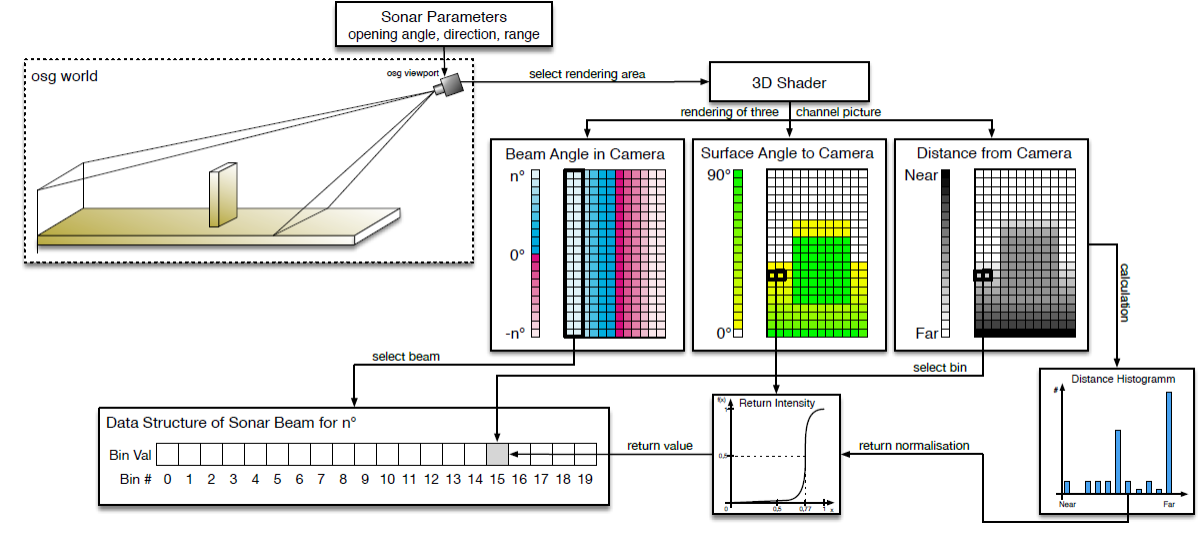
\includegraphics[scale=0.35]{dados/figuras/gpu_sonar.png}
    \fonte{\cite{cerqueira2016gpu}.}
\end{figure}

Esses parâmetros afetam no processamento do simulador e resolução da imagem. Quanto maior o número de \textit{bins}, melhor será a qualidade da imagem acústica. A Figura \ref{fig:gpu_sonar_sim} ilustra o método utilizado no simulador e descrito nessa seção.

\section{\textit{Point Cloud Library}}
\label{sec:pcl}

A PCL (Biblioteca de Nuvem de Pontos, do inglês \textit{Point Cloud Library}) é um \textit{framework} para o processamento de imagens e nuvens de pontos em 2D/3D desenvolvido para a linguagem \textit{C++}. 
O \textit{framework} é um projeto de código aberto em larga escala criado por \cite{rusu2011pcl}. 
A PCL contém diversos algoritmos no estado da arte, incluindo filtros, estimação de \textit{features}, reconstrução de superfícies, segmentação, entre outros. 
Em paralelo, \cite{strawlab2012} adaptou parte da PCL para a linguagem python. 

\begin{figure}[H]
    \centering
    \caption{Exemplo de utilização da PCL em dados adquiridos por um sensor a laser.}
    \label{fig:pcl_example}
    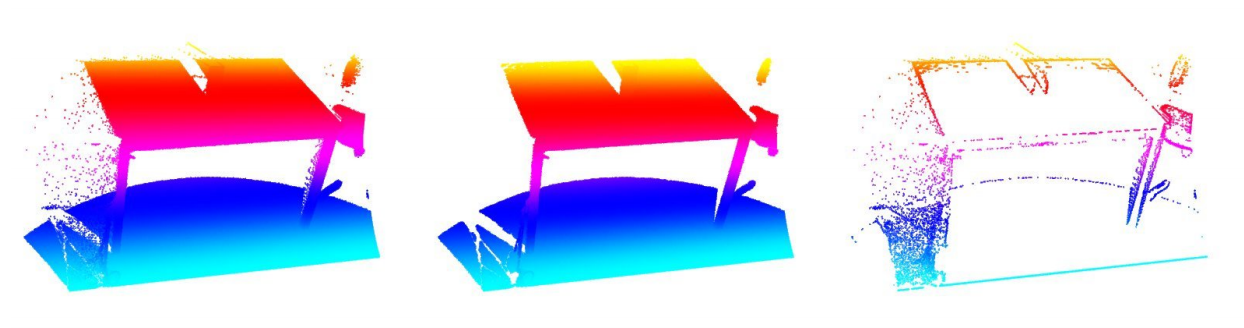
\includegraphics[scale=0.3]{dados/figuras/pcl_example.png}
    \fonte{\cite{rusu2011pcl}.}
\end{figure}

A Figura \ref{fig:pcl_example} ilustra um exemplo da aplicação da PCL em uma nuvem de pontos. Na imagem a esquerda mostra uma nuvem de pontos adquirida a partir de um sensor a laser, a imagem do meio mostra a nuvem resultante após passar por um filtro\footnote{O filtro utilizado se chama \textit{StatisticalOutlierRemoval} (filtro estatístico de remoção de \textit{outliers}) descrito na Seção \ref{sec:statical_outlier_removal}. A documentação do filtro se encontra em: \url{http://pointclouds.org/documentation/tutorials/statistical_outlier.php}.}, por último, os pontos descartados são mostrados na figura na direita.         % Fundamentação Teórica
% METODOLOGIA------------------------------------------------------------------

\chapter{METODOLOGIA}
\label{chap:metodologia}

A metodologia do trabalho é composta por duas partes, onde a primeira é a coleta de dados e, a segunda, o desenvolvimento da aplicação. 
Na segunda parte da execução do trabalho, será o desenvolvimento do algoritmo de reconstrução, que consistirá em quatro etapas, no qual, para cada etapa é desenvolvido uma rotina. 
Primeiro os dados serão preparados, em seguida serão refinados e filtrados, por fim, renderizados.
O resultado final do processamento, será uma superfície tridimensional.
Cada parte está segmentada em etapas, no qual cada etapa é um processo a ser executado. Por conseguinte, a organização da metodologia apresenta os itens:

\begin{itemize}
    \addtolength{\itemindent}{2em}
    
    \item Coleta de dados:
    \begin{itemize}
        \addtolength{\itemindent}{2em}
        
        \item Dados em simulação;
        \item Dados \textit{in loco}.
    \end{itemize}
    
    \item Desenvolvimento:
    \begin{itemize}
        \addtolength{\itemindent}{2em}
        
        \item Pré-processamento;
        \item Filtragem;
        \item Reconstrução;
        \item Comparação.
    \end{itemize}
\end{itemize}
\hspace{1em}

A Figura \ref{fig:etapas} mostra as etapas do desenvolvimento da aplicação. Primeiramente, os dados são inseridos através de um \textit{dataset}. 
Em verde são representados as etapas do pré-processamento.
Em amarelo são representados os processos de filtragem.
O último processo é o de reconstrução, onde ocorre a reconstrução, representado em marrom.
A etapa de comparação, é um processo a parte do fluxo principal, no qual requer duas superfícies na entrada do processo para gerar a superfície resultante.


\begin{figure}[H]
    \centering
    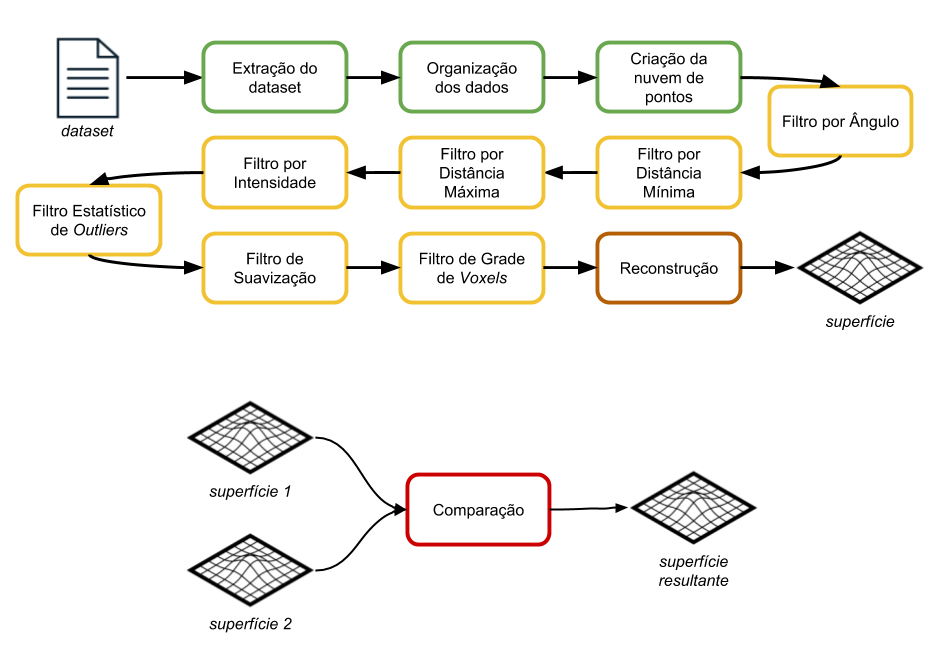
\includegraphics[scale=0.4]{dados/figuras/etapas.png}
    \caption{Etapas da metodologia proposta.}
    \label{fig:etapas}
\end{figure}

\section{Coleta de dados}
\label{sec:coleta_dados}

A coleta de dados foi realizada de duas formas: em simulação virtual e \textit{in loco}. 
A coleta em simulação virtual facilita a obtenção de dados, por não haver a necessidade de possuir um sensor ou robô e por dispensar planejamento logístico que uma saída de campo requer. 
Contudo, é importante fazer a coleta \textit{in loco}, pois possibilita realizar a comparação do desempenho do algoritmo e, além disso, as informações obtidas serão mais próximas do mundo real quanto às coletadas em simulação.

\subsection{Simulação virtual}
\label{sec:simulation}

A obtenção de dados por simulação virtual contará com o auxílio de \textit{softwares} e ferramentas. 
O \textit{software} Gazebo será o responsável por simular o ambiente virtual, enquanto que o ROS será responsável por executar o modelo do veículo ROV e o simulador do sonar MSIS.
O veículo ROV utilizado, chamado RexROV (Figura \ref{fig:rexrov}), foi desenvolvido pelos autores \cite{manhaes2016uuv} e está incluso no pacote \textit{UUV Simulator}.
Os sensores utilizados pelo RexROV e sua estrutura são semelhantes ao ROV utilizado (Figura \ref{fig:rov_nautec}) nos experimentos reais.
O ambiente de simulação, apresentado na Figura \ref{fig:environment}, representa o fundo de um corpo d'água.
Assim como o robô, o ambiente de simulação também está disponível no pacote \textit{UUV Simulator}.

\begin{figure}[H]
    \centering
    \begin{subfigure}[t]{0.4\textwidth}
        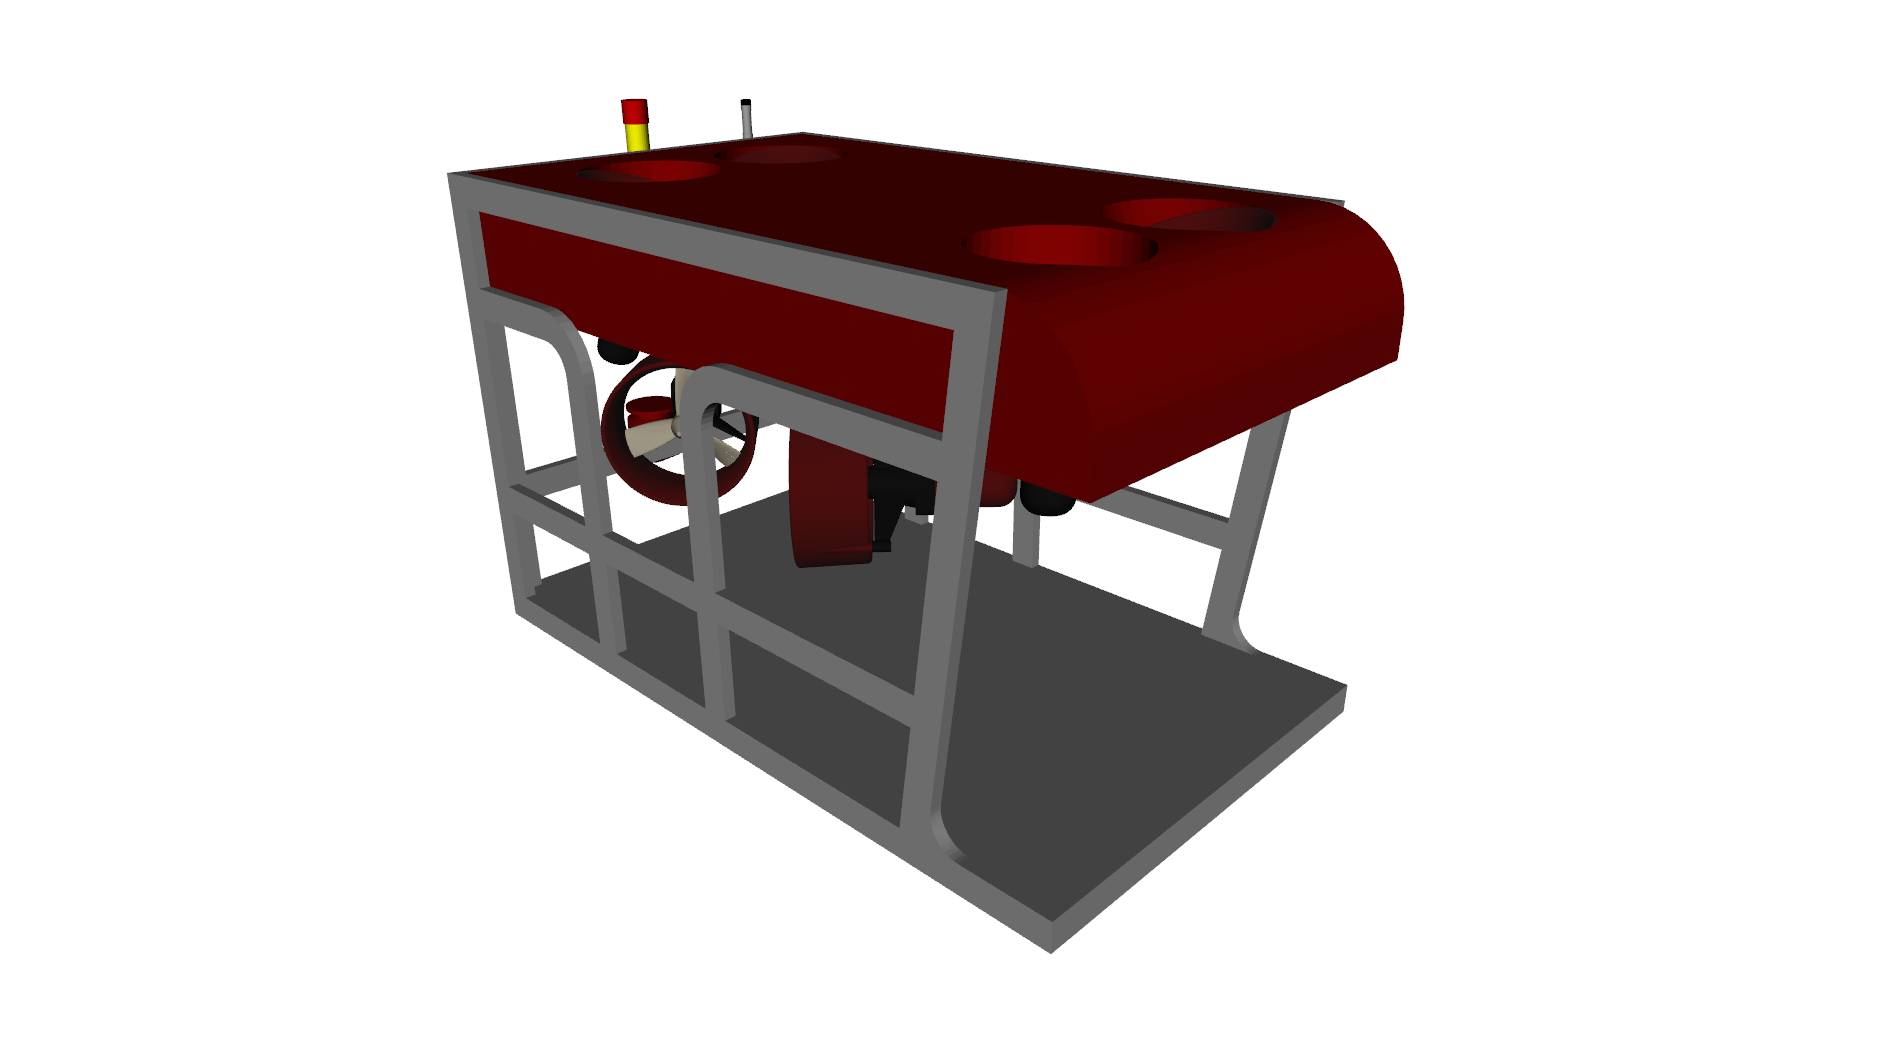
\includegraphics[width=\textwidth]{dados/figuras/rexrov.png}
        \caption{Veículo RexROV.}
        \label{fig:rexrov}
    \end{subfigure}
    \hspace{1em}
    \begin{subfigure}[t]{0.55\textwidth}
        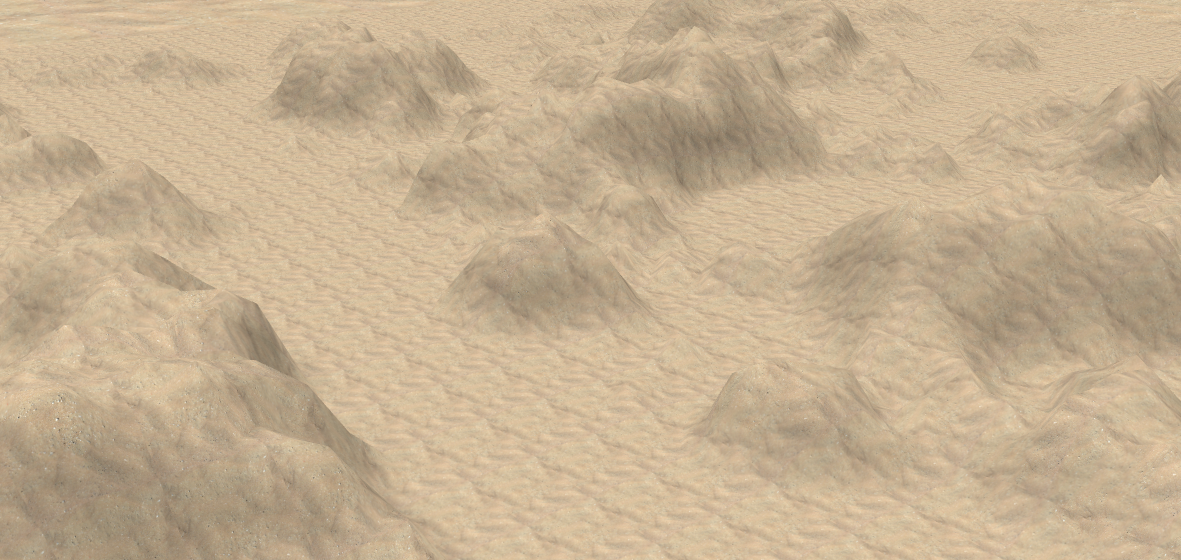
\includegraphics[width=\textwidth]{dados/figuras/environment.png}
        \caption{Ambiente em simulação.}
        \label{fig:environment}
    \end{subfigure}
    \caption{Veículo e ambiente utilizado na simulação virtual.}
    \label{fig:simulation}
\end{figure}

Em simulação, as unidades utilizadas para o comprimento não estão definidas em metros, por esse motivo qualquer comprimento descrito no ambiente de simulação será na sigla \textit{uc} (unidades de comprimento).
No ambiente, como mostra a Figura \ref{fig:scenaries}, foi acrescentado obstáculos para montar diferentes tipos de cenários.
Nos cenários A e B foram acrescentadas a mesma parede, a diferença está na posição no segundo cenário, que está 5uc mais distante em relação ao primeiro cenário.

\begin{figure}[H]
    \centering
    \begin{subfigure}[t]{0.328\textwidth}
        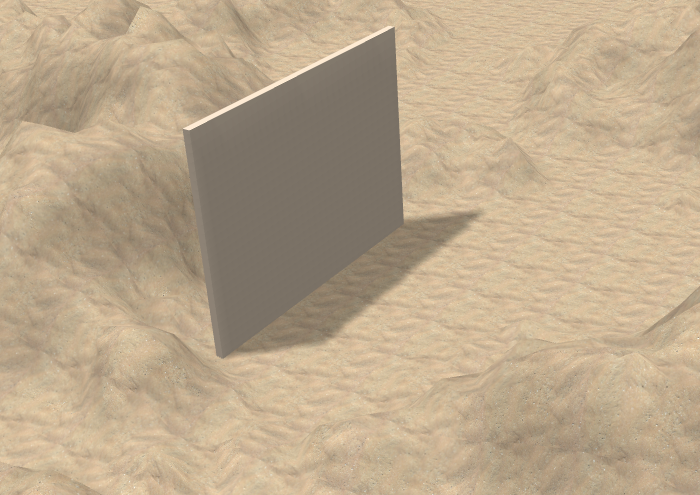
\includegraphics[width=\textwidth]{dados/figuras/scene3.png}
        \caption{}
        \label{fig:scene2}
    \end{subfigure}
    \begin{subfigure}[t]{0.328\textwidth}
        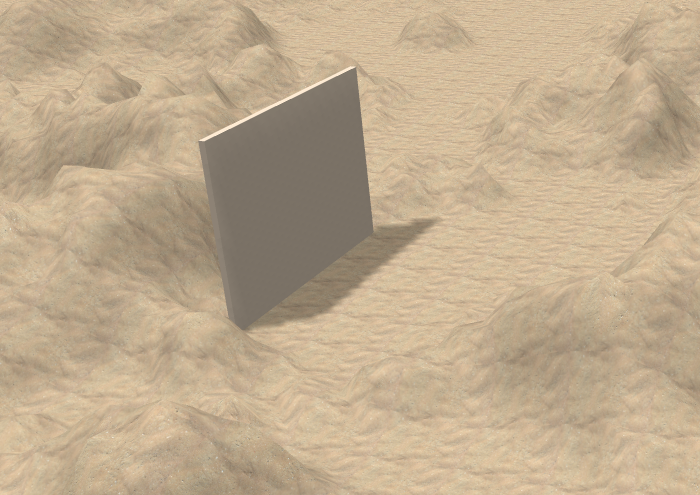
\includegraphics[width=\textwidth]{dados/figuras/scene2.png}
        \caption{}
        \label{fig:scene1}
    \end{subfigure}
    \begin{subfigure}[t]{0.328\textwidth}
        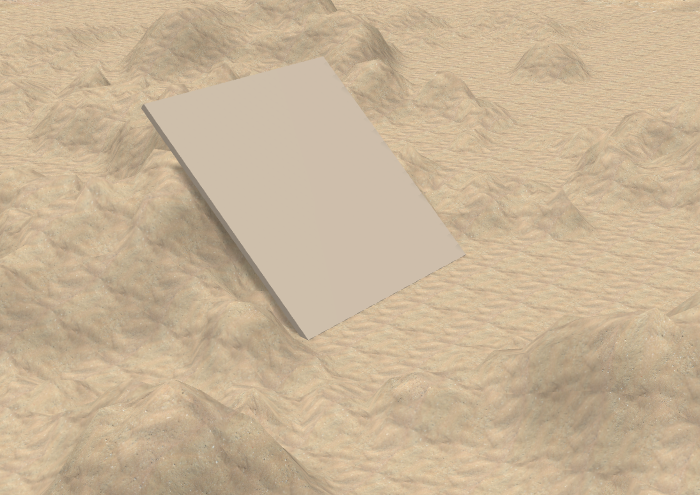
\includegraphics[width=\textwidth]{dados/figuras/scene4.png}
        \caption{}
        \label{fig:scene3}
    \end{subfigure}
    \caption{Cenários criados para realizar o experimento.}
    \label{fig:scenaries}
\end{figure}

O cenário C foi construído a partir do cenário A, onde ocorre a inclinação em 45º da parede e alongamento da sua altura para manter a mesma da parede do cenário anterior.
A intenção é simular uma geleira em um estado inicial, representado pelo cenário A, e em um estado posterior após perder o volume inicial, representado pelos cenários B e C.
Portanto, a comparação de volume acontecerá em dois contextos: o primeiro contexto será chamado de AB, onde os cenários A e B estão envolvidos, no qual simula uma perda de volume, pois A está 5uc à frente de B; o segundo contexto será chamado de AC, onde os cenários A e C estão envolvidos, no qual há uma perda maior de volume em relação ao primeiro contexto.
O contexto é um cenário onde há dois modelos reconstruídos, que serve para fazer a comparação entre esses modelos.
A Figura \ref{fig:dimensoes} exibe as dimensões das paredes utilizadas nas simulações.

\begin{figure}[H]
    \centering
    \begin{subfigure}[t]{0.328\textwidth}
        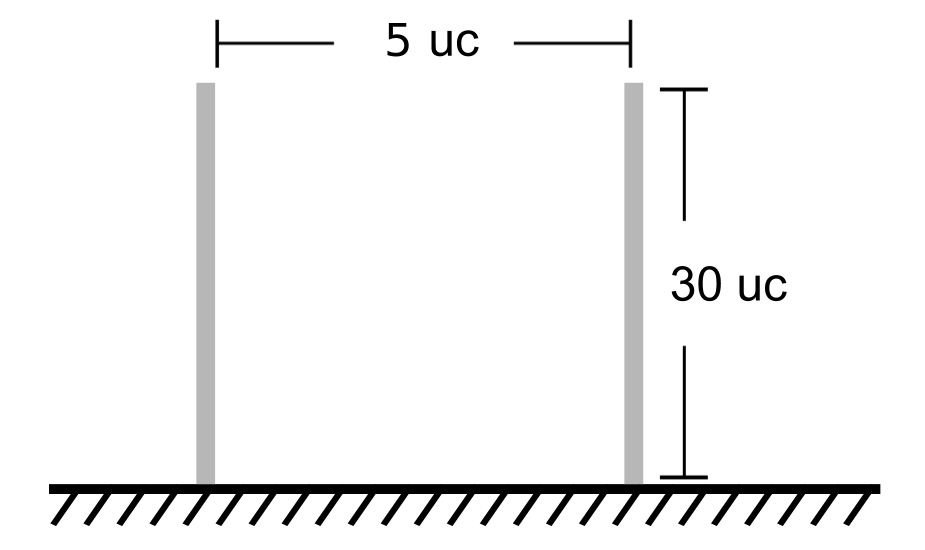
\includegraphics[width=\textwidth]{dados/figuras/dim_lateral_ab.png}
        \caption{Vista lateral entre \textbf{a} e \textbf{b}.}
        \label{fig:dim_lateral_ab}
    \end{subfigure}
    \begin{subfigure}[t]{0.328\textwidth}
        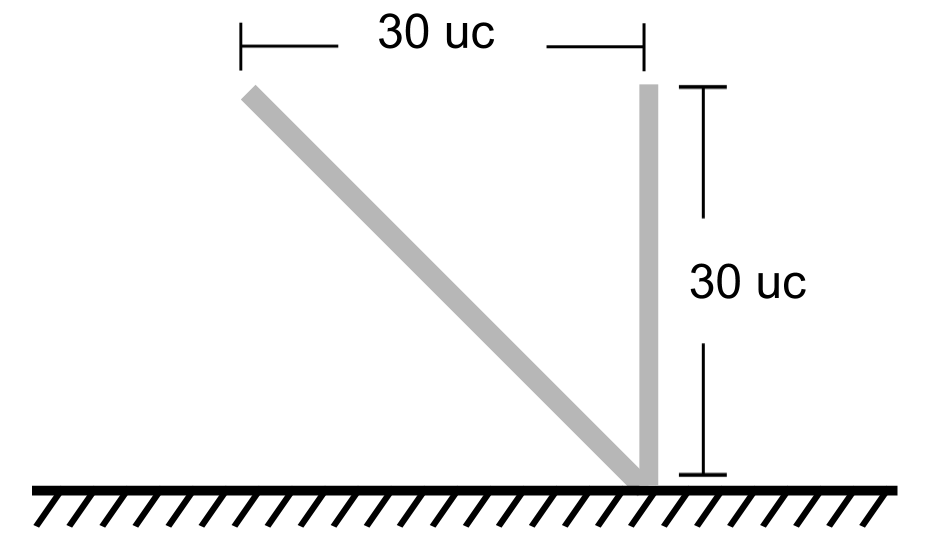
\includegraphics[width=\textwidth]{dados/figuras/dim_lateral_ac.png}
        \caption{Vista lateral entre \textbf{a} e \textbf{c}.}
        \label{fig:dim_lateral_ac}
    \end{subfigure}
    \begin{subfigure}[t]{0.328\textwidth}
        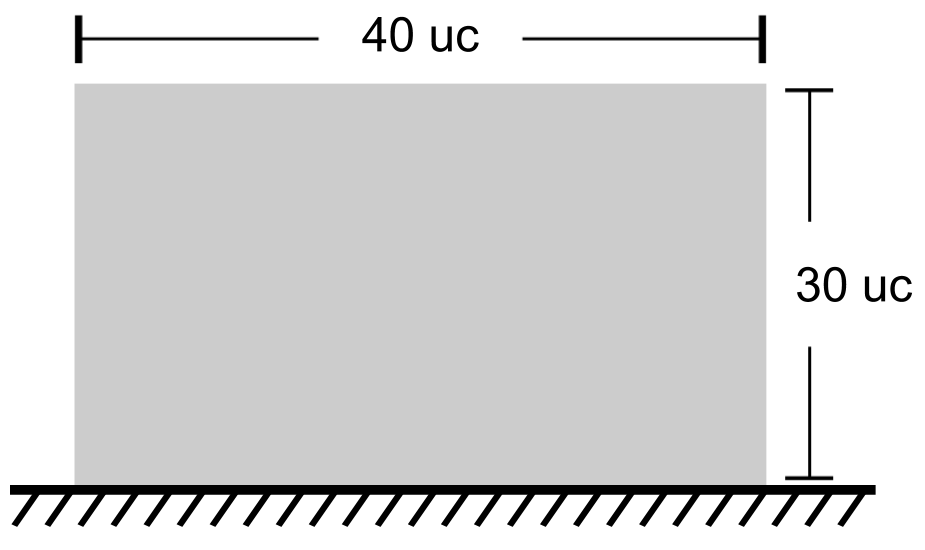
\includegraphics[width=\textwidth]{dados/figuras/dim_frontal.png}
        \caption{Vista frontal da parede.}
        \label{fig:dim_frontal}
    \end{subfigure}
    \caption{Dimensões das paredes.}
    \label{fig:dimensoes}
\end{figure}

Em todos os \textit{datasets} criados, o ROV foi posicionado a uma distância de aproximadamente 25uc, iniciando a coleta na parte superior da superfície. 
Após o início, o sensor faz a leitura completa de uma imagem acústica, ou seja, o transdutor percorrer de 0º à  180º, gerando um \textit{beam} por grau.
Realizada a coleta de uma imagem acústica, o robô ativa os propulsores para se deslocar cerca de 0.7uc em direção ao solo. 
Após o deslocamento, o processo de leitura se repete até o veículo encostar no leito do corpo d'água.


\subsection{Aquisição \textit{in loco}}
\label{sec:in_loco}

A aquisição de dados em campo foi realizada em uma piscina, como mostra a Figura \ref{fig:piscina}.
A piscina possui o formato de um retângulo no qual há dois lados maiores e dois lados menores, onde foi utilizado apenas um dos lados menores.

O ROV foi posicionado inicialmente à uma determinada distância da parede e próximo a superfície.
O sensor faz a leitura da parede, percorrendo 180º e na sequência se desloca alguns centímetros verticalmente em direção ao fundo.
Esse procedimento se repete até o robô encostar no fundo da piscina.
No primeiro experimento, chamado de cenário D, o ROV foi posicionado a 1,5 metros de distância da parede da piscina.
Após concluir a varredura, o procedimento é repetido, porém à uma distância de 3 metros, esse será o cenário E. 
Ambos cenários vão compor o único contexto do experimento em campo.

\iffalse
O segundo experimento foi semelhante ao primeiro, porém foi realizado no outro lado, no qual possui uma escadaria, e as distâncias eram de 2,5 e 4 metros.
O cálculo de volume só haverá no primeiro experimento, pois no segundo, não há como saber o real valor do volume da escadaria.
\fi

\begin{figure}[H]
    \centering
    \begin{subfigure}[t]{0.22\textwidth}
        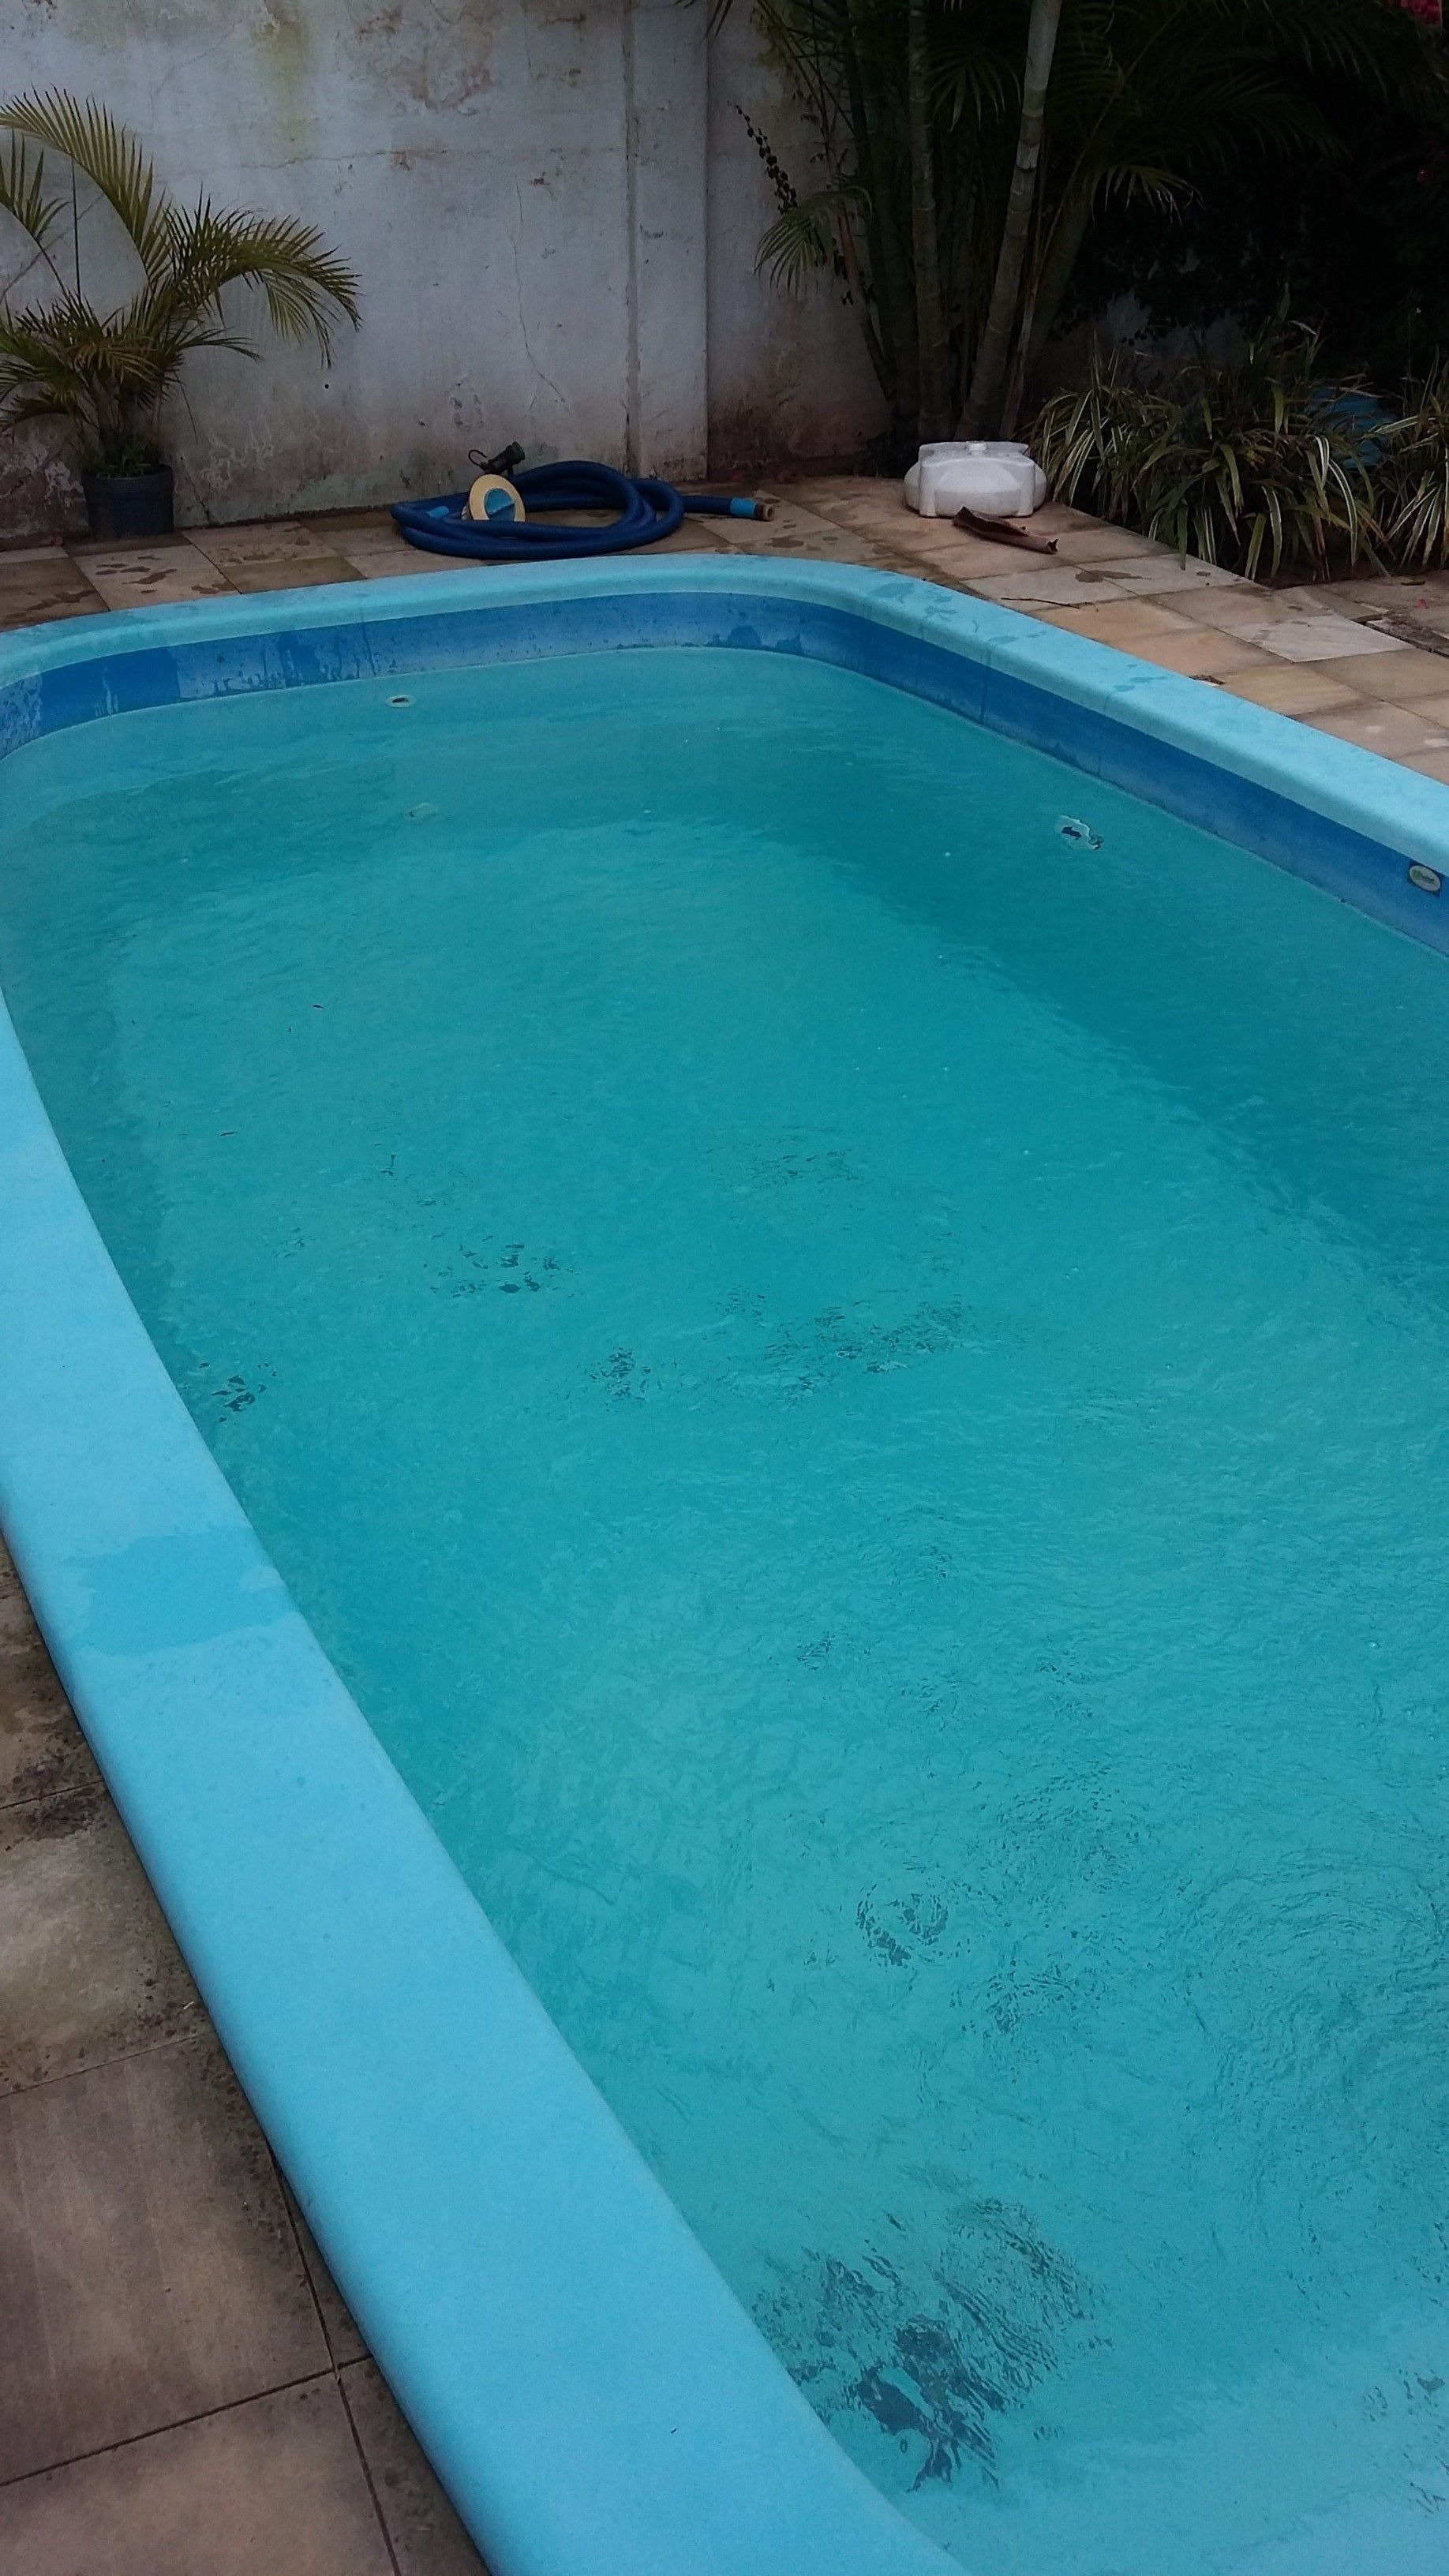
\includegraphics[width=\textwidth]{dados/figuras/piscina_1.jpg}
    \end{subfigure}
    \hspace{1em}
    \begin{subfigure}[t]{0.22\textwidth}
        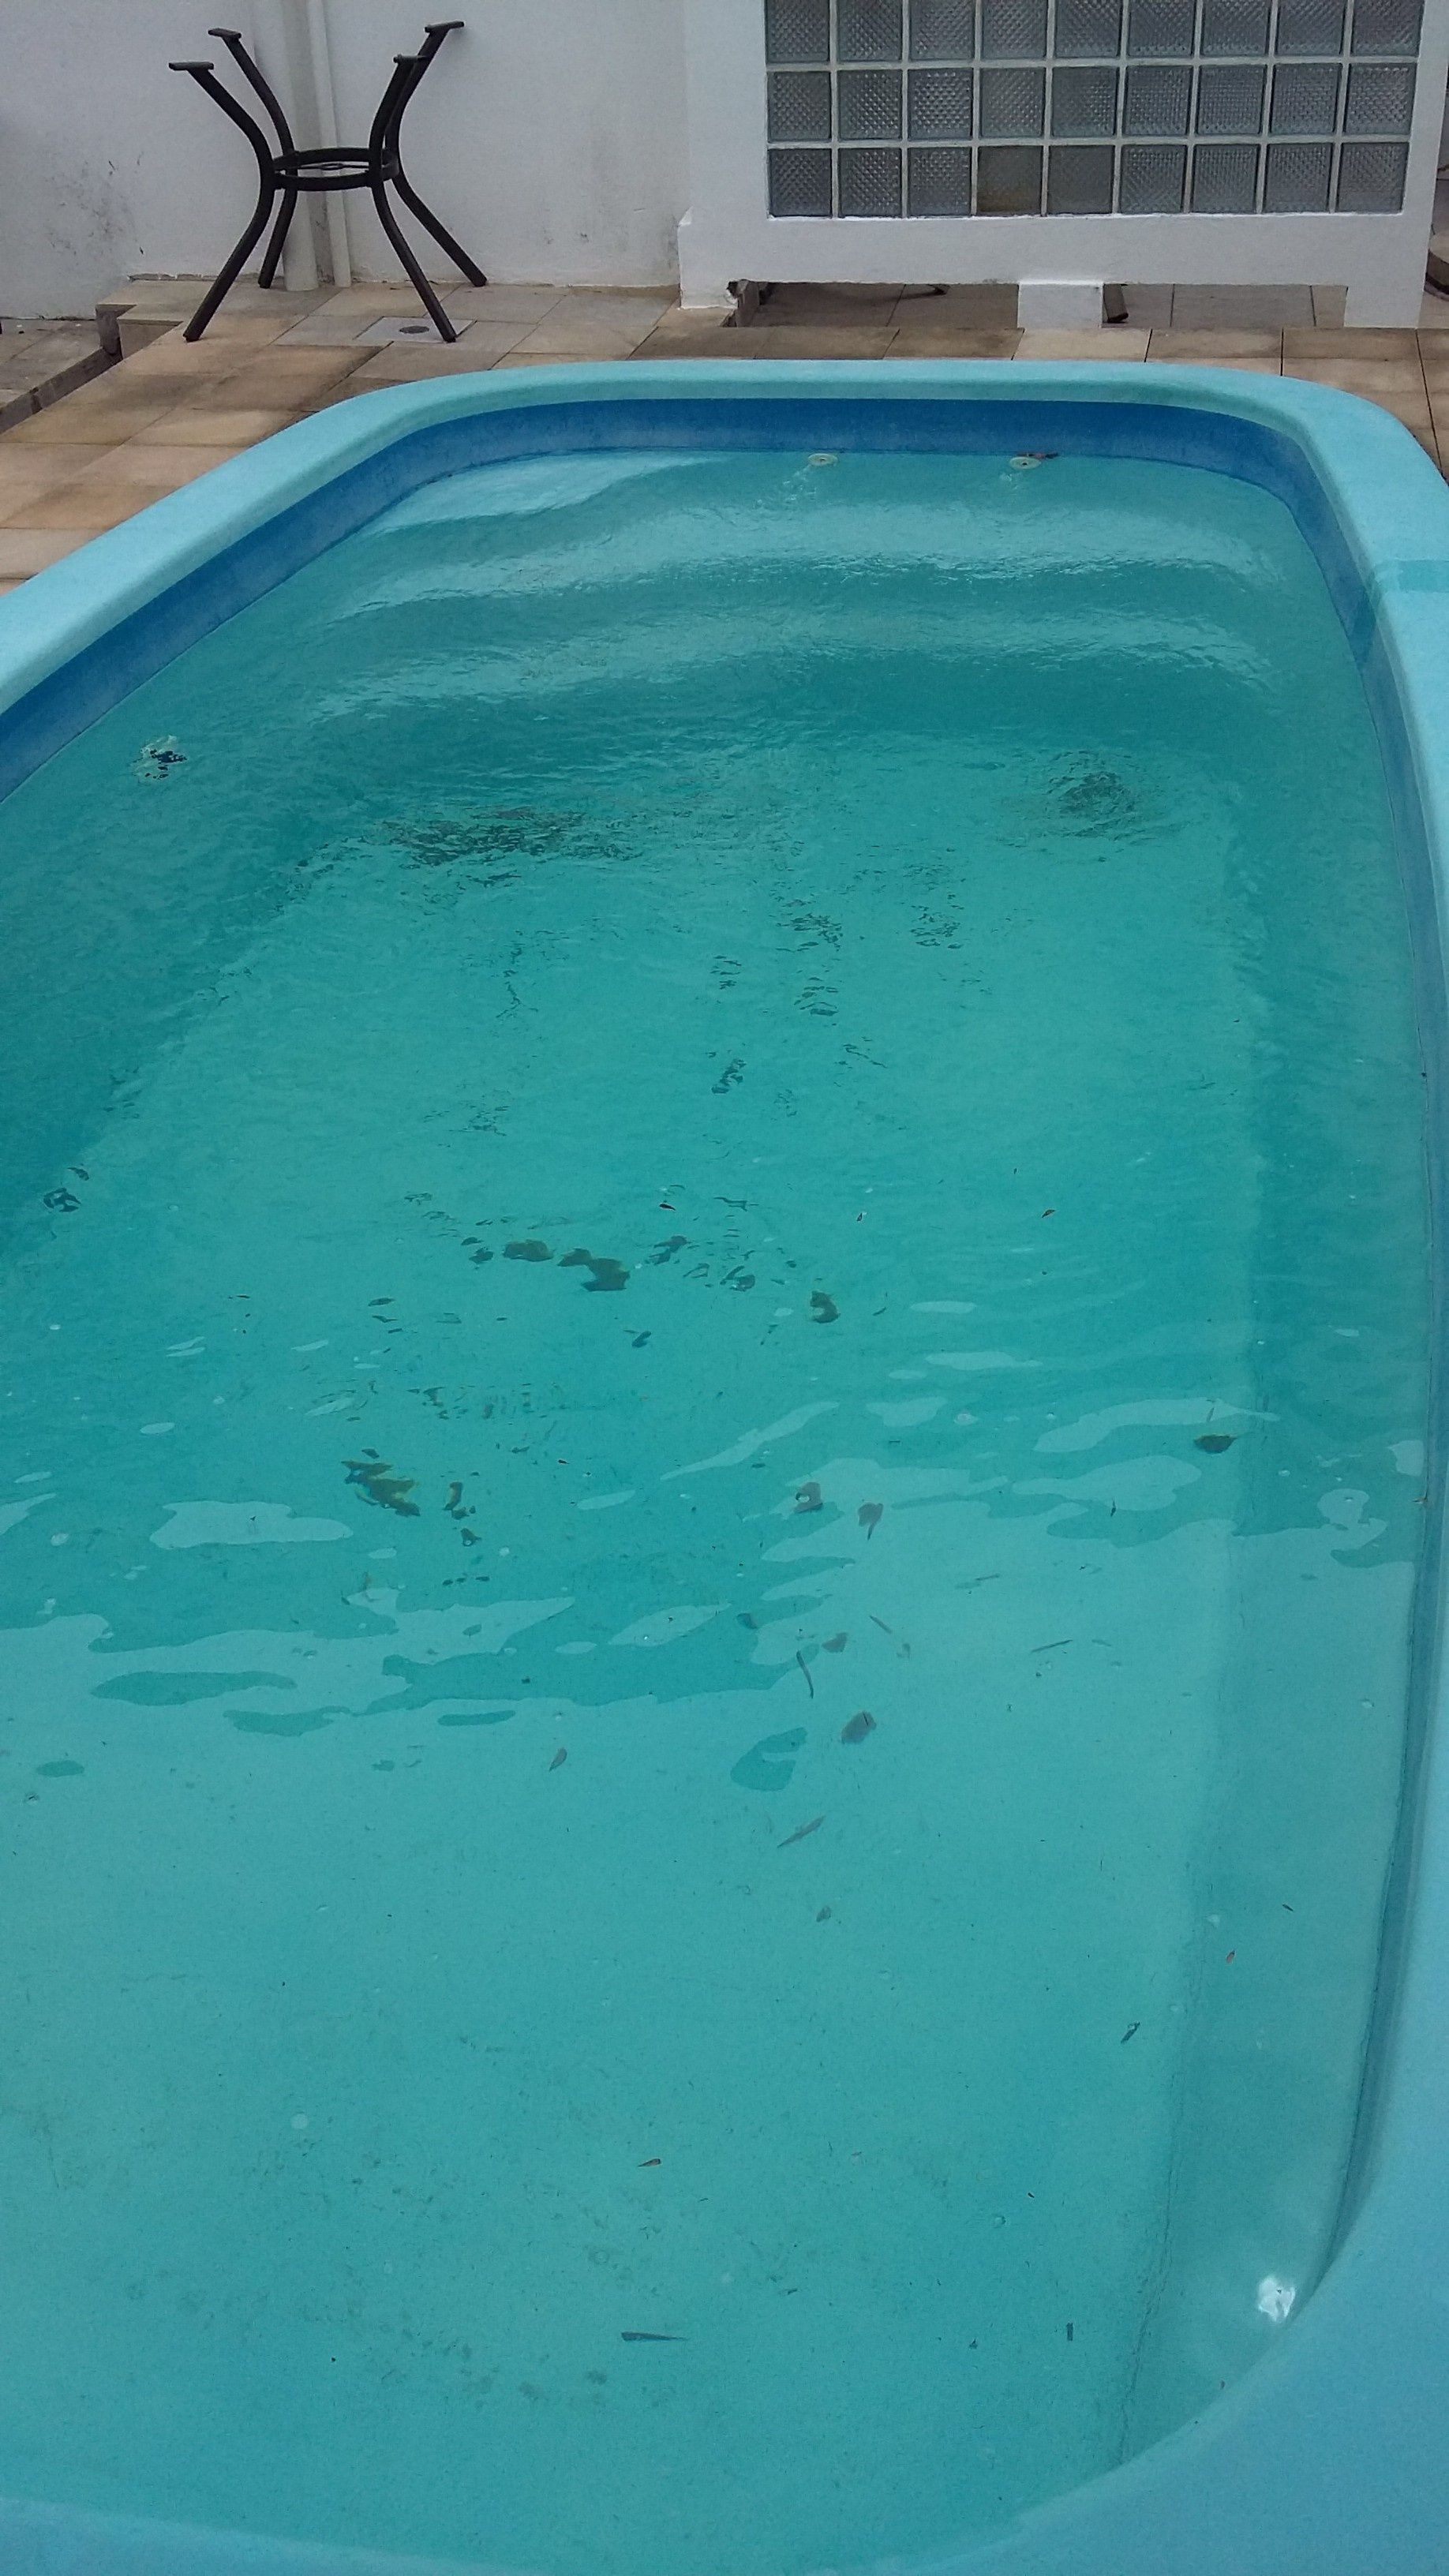
\includegraphics[width=\textwidth]{dados/figuras/piscina_2.jpg}
    \end{subfigure}
    \caption{Piscina onde foi realizado o experimento.}
    \label{fig:piscina}
\end{figure}

Para fazer a coleta, foi utlizado o ROV, modelo LBV300-5 da SeaBotix\footnote{Informações completas do modelo do ROV no Anexo \ref{chap:especificacao_rov}.} (Figura \ref{fig:rov_nautec}), do grupo NAUTEC do C3. 
Acoplado ao robô, será utilizado o sensor MSIS modelo Tritech Micron Sonar\footnote{Informações completas do modelo do sensor no Anexo \ref{chap:especificacao_sonar}.} que é responsável pela captura dos dados.

\begin{figure}[H]
    \centering
    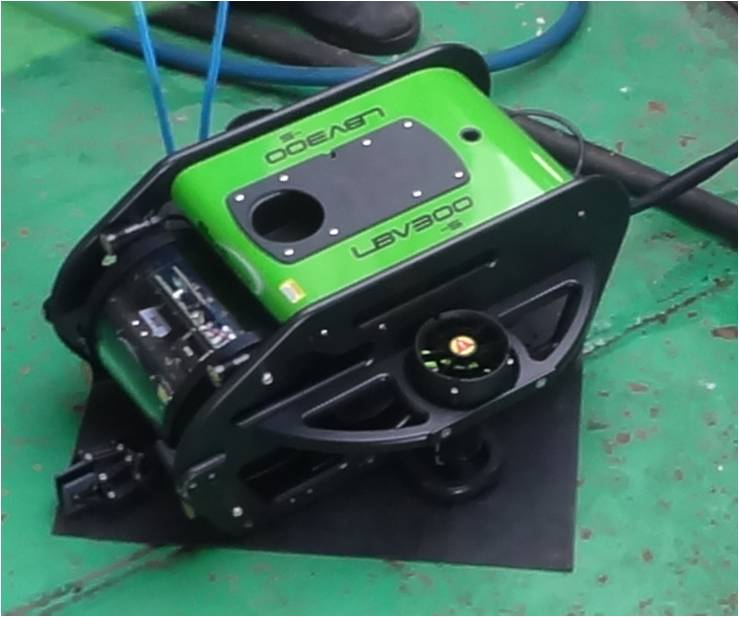
\includegraphics[scale=0.5]{dados/figuras/rov_furg.jpg}
    \caption{ROV utilizado no trabalho.}
    \label{fig:rov_nautec}
\end{figure}

\section{Pré-processamento}

A etapa de pré-processamento serve para manipular os dados do \textit{dataset} e dispor em uma nuvem de pontos.
No final da fase de pré-processamento, o produto gerado é uma nuvem de pontos da superfície que foi escaneada pelo sonar. Esse resultado servirá como entrada para o próximo processo.

Nessa etapa, ocorre a escolha dos \textit{bins} que vão compor cada imagem.
Deve ser selecionado um \textit{bin} por cada \textit{beam} da imagem acústica.
O critério utilizado será o critério que escolhe o \textit{bin} com o maior sinal de intensidade do \textit{beam}.

\begin{figure}[H]
    \centering
    \begin{subfigure}[t]{0.45\textwidth}
        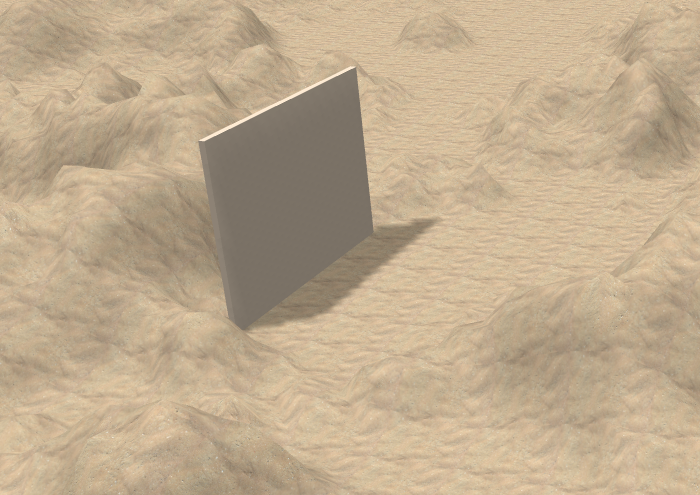
\includegraphics[width=\textwidth]{dados/figuras/scene2.png}
        \caption{Ambiente em simulação virtual.}
        \label{fig:point_cloud_example_a}
    \end{subfigure}
    \begin{subfigure}[t]{0.45\textwidth}
        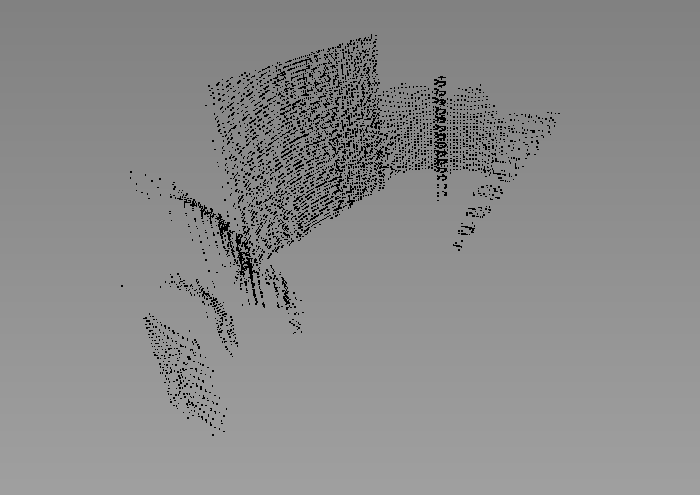
\includegraphics[width=\textwidth]{dados/figuras/point_cloud.png}
        \caption{Nuvem de pontos gerada.}
        \label{fig:point_cloud_example_b}
    \end{subfigure}
    \caption{Nuvem de pontos gerada a partir de dados coletados em simulação virtual por um sonar MSIS.}
    \label{fig:point_cloud_example}
\end{figure}

Na Figura \ref{fig:point_cloud_example} mostra o ambiente em simulação escaneado pelo sonar e a nuvem de pontos gerada.
A etapa de pré-processamento não é responsável por filtrar a nuvem de pontos, por esse motivo que a nuvem gerada na Figura \ref{fig:point_cloud_example_b} possui uma grande quantidade de ruído.


\section{Filtragem}
\label{sec:filtragem}

O processo de filtragem ou \textit{denoising} é composto por um conjunto de filtros em forma de funções que tem como objetivo remover ou atenuar informações desnecessárias da nuvem de pontos, como ruídos e \textit{outliers}\footnote{\textit{Outliers} é um termo da área da estatística utilizado para referênciar elementos atípicos ou observações que estão muito afastadas do restante da série.}.
Além disso, o objetivo é facilitar o processo de reconstrução e de cálculo de volume.
O resultado da etapa de filtragem é uma nuvem de pontos mais limpa e legível, porém o processo de filtragem nem sempre é capaz de remover todas as informações desnecessárias.

\begin{figure}[H]
    \centering
    \begin{subfigure}[t]{0.49\textwidth}
        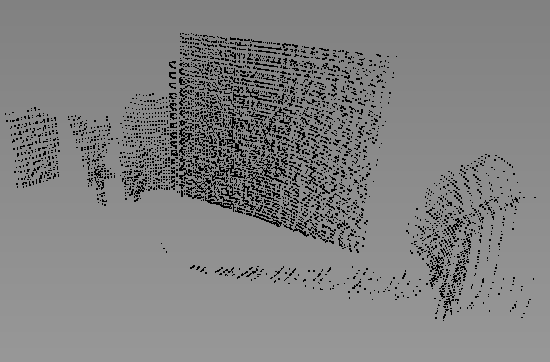
\includegraphics[width=\textwidth]{dados/figuras/pc_noise.png}
        \caption{Nuvem de pontos com ruído.}
    \end{subfigure}
    \begin{subfigure}[t]{0.49\textwidth}
        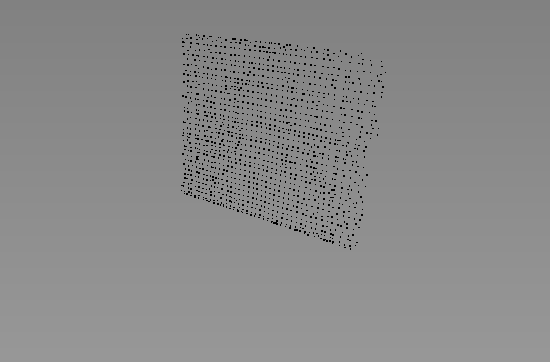
\includegraphics[width=\textwidth]{dados/figuras/pc_denoise.png}
        \caption{Nuvem de pontos após a remoção de ruído.}
    \end{subfigure}
    \caption{Processo de remoção de ruído em uma nuvem de pontos.}
    \label{fig:point_cloud_denoise}
\end{figure}

Para realizar essa etapa, os filtros foram separados em dois grupos.
O primeiro grupo é composto por filtros simples, porém removem maior parte dos pontos desnecessários. 
O segundo conjunto é formado por filtros complexos onde todos já estão implementados na PCL (Seção \ref{sec:pcl}).
Os filtros simples são representados pelo filtro por ângulo, filtro por intensidade, filtro por distância máxima e filtro por distância mínima, enquanto que os filtros complexos, são retratados pelo Filtro de Grade de \textit{Voxels}\footnote{Um \textit{voxel} é um \textit{pixel} que contém volume em um espaço tridimensional. Fazendo uma analogia, o \textit{voxel} seria um \textit{pixel} em 3D.}, Filtro de Suavização e o Filtro Estatístico de Remoção de \textit{Outliers}.


\subsection{Filtro por ângulo}
\label{sec:angle_filter}

O filtro por ângulo, remove qualquer ponto que está fora da área cônica definida pelo ângulo horizontal $\theta$. Para esclarecer, na nuvem de pontos da Figura \ref{fig:angle_filter} são mostrados em cinza e em preto, os pontos descartados e mantidos pelo filtro, respectivamente.
O ângulo de abertura no sensor geralmente é configurável no próprio hardware, porém o critério do descarte fica por conta da aplicação, pois em um \textit{dataset}, os mesmos pontos que são inúteis em um trabalho podem ser úteis em outro. 
Por padrão, foi utilizado 120 graus para o ângulo $\theta$.

\subsection{Filtro por distância mínima}
\label{sec:distance_filter}

O filtro por distância mínima faz a remoção de pontos que estão próximos ao sensor, onde a presença de ruído costuma ser elevada. 
Da mesma forma como abordado no filtro anterior, os pontos em cinzas são descartados enquanto que os pretos são mantidos, como mostra a Figura \ref{fig:distance_filter}. 
Por padrão, o valor adotado para o raio de exclusão é de 5\textit{uc}, ou seja, serão descartados todos os pontos que estiverem até 5uc de distância do sensor.

\subsection{Filtro por distância máxima}
\label{sec:distance_filter2}

O filtro por distância máxima funciona da mesma forma que o filtro por distância mínima, porém se faz a remoção de pontos que estão distantes do sensor (Figura \ref{fig:distance_filter2}).
Ele é utilizado apenas nos dados coletados no experimento \textit{in loco}, onde a presença de ruído é alta em pontos distantes por conta da reverberação (descrito na Seção \ref{sec:imagem_acustica}).

\subsection{Filtro por intensidade}
\label{sec:intensity_filter}

Este processo remove os pontos que possuem baixo valor de intensidade. Os motivos para o sinal de intensidade ser baixo em um determinado ponto, pode ser:
    \begin{itemize}
        \item O ponto estar distante do sensor. Nesse caso, o sinal da onda estará fraco ao entrar em contato com o ponto, por conta da perda de energia para o meio ao longo da distância percorrida;
        \item O ângulo de incidência da onda com o ponto ser obtuso. Quando menos ortogonal o ângulo de incidência entre a onda e o ponto, mais fraco será o sinal de retorno;
        \item A composição do objeto detectado pela onda. Quanto mais denso for o objeto, maior será o sinal de retorno.
    \end{itemize}

\begin{figure}[H]
    \centering
    \begin{subfigure}[t]{0.4\textwidth}
        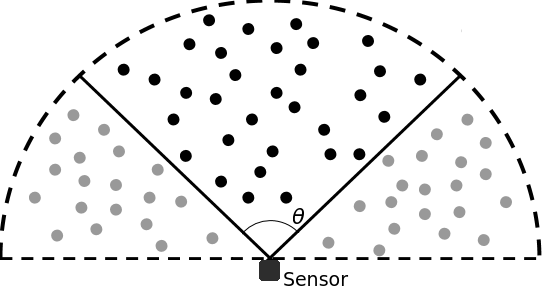
\includegraphics[width=\textwidth]{dados/figuras/angle_filter.png}
        \caption{Filtro por ângulo horizontal.}
        \label{fig:angle_filter}
    \end{subfigure}
    \hspace{3em}
    \begin{subfigure}[t]{0.4\textwidth}
        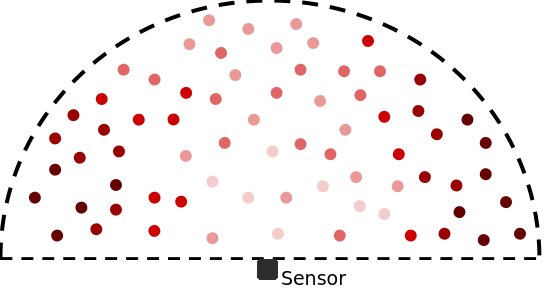
\includegraphics[width=\textwidth]{dados/figuras/intensity_filter.png}
        \caption{Filtro por intensidade.}
        \label{fig:intensity_filter}
    \end{subfigure}
    \begin{subfigure}[t]{0.4\textwidth}
        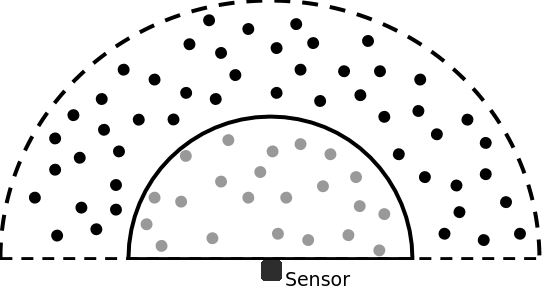
\includegraphics[width=\textwidth]{dados/figuras/distance_filter.png}
        \caption{Filtro por distância mínima.}
        \label{fig:distance_filter}
    \end{subfigure}
    \hspace{3em}
    \begin{subfigure}[t]{0.4\textwidth}
        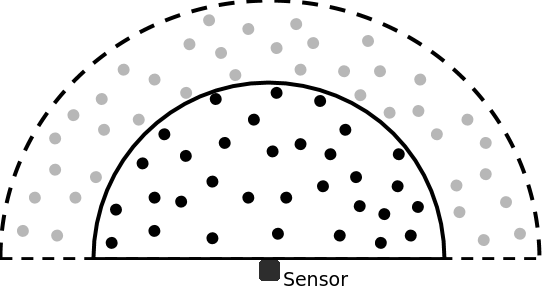
\includegraphics[width=\textwidth]{dados/figuras/distance_filter2.png}
        \caption{Filtro por distância máxima.}
        \label{fig:distance_filter2}
    \end{subfigure}
    \caption{Filtros simples de remoção de \textit{outliers}.}
\end{figure}

O exemplo ilustrado na Figura \ref{fig:intensity_filter}, mostra uma nuvem onde os pontos possuem diversos valores de intensidade. 
Quanto mais claro for o ponto, maior será o seu valor de intensidade do sinal de retorno. 
Portanto, o filtro descarta os pontos mais escuros na imagem.
Por padrão, é descartado todos os pontos que possuírem o valor de intensidade igual ou menor que 5\% da diferença entre o valor máximo e o valor mínimo de intensidade da nuvem de pontos.

\subsection{Filtro de grade de \textit{voxels}}
\label{sec:voxelgrid_filter}

O Filtro de Grade de \textit{Voxels} (do inglês \textit{Voxel Grid Filter}) tem a finalidade de uniformizar a densidade e ordenar os pontos em uma nuvem. 
A Figura \ref{fig:voxelgrid_filter} exibe uma nuvem de pontos de entrada (esquerda) e o resultado gerado após aplicar o filtro (direita).

\begin{figure}[H]
    \centering
    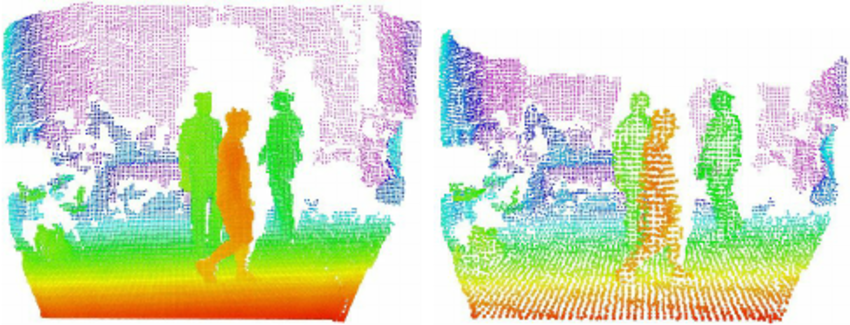
\includegraphics[scale=0.4]{dados/figuras/voxelgrid_filter.png}
    \caption{Exemplo da aplicação do Filtro de Grade de \textit{Voxels}.}
    \vspace{-0.8em}
    \fonte{\cite{munaro2012tracking}.}
    \label{fig:voxelgrid_filter}
\end{figure}

Para diminuir a quantidade de pontos e ordená-los, o algoritmo cria uma grade no conjunto de dados, onde os pontos são deslocados para o centroide da célula (\textit{voxel}) da grade em que estão contidos (o tamanho do \textit{voxel} é definido pelo usuário). A diminuição da quantidade e ordenação dos pontos facilita o processo de triangularização (etapa posterior responsável por transformar a nuvem de pontos em uma superfície).

\subsection{Filtro estatístico de remoção de \textit{outliers}}
\label{sec:statistical_outlier_removal}

O SORF (Filtro Estatístico de Remoção de \textit{Outliers}, do inglês \textit{Statistical Outlier Removal Filter}) é um filtro da biblioteca PCL que é responsável por remover conjuntos de pontos que possuem uma densidade menor do que o restante dos conjuntos de pontos dentro da nuvem. 
A Figura \ref{fig:outlier_filter} exemplifica a aplicação do filtro. Na imagem à esquerda mostra a nuvem original que contém regiões em destaque, onde a densidade de pontos é menor que no restante da nuvem, enquanto que na imagem à direita mostra a remoção desses conjuntos de pontos.

\begin{figure}[H]
    \centering
    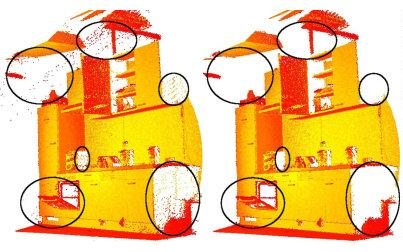
\includegraphics[scale=0.6]{dados/figuras/outlier_filter.jpg}
    \caption{Exemplo de uso do SORF.}
    \vspace{-0.8em}
    \fonte{Adaptado de \cite{rusu2011pcl}.}
    \label{fig:outlier_filter}
\end{figure}

O filtro percorre a nuvem calculando, para cada ponto, a distância média entre seus pontos vizinhos (o número de vizinhos é definido pelo usuário). Assumindo o resultado como uma distribuição Gaussiana com uma média e um desvio padrão, todos os pontos cuja distância média estão fora de um intervalo definido pela média das distâncias globais e desvio padrão podem ser considerados \textit{outliers} e, portanto, removidos do conjunto de dados.

\subsection{Filtro de suavização}
\label{sec:smoothing_filter}

O Filtro de Suavização é um filtro que está presente na biblioteca PCL e é responsável por suavizar e reconstruir a superfície de pontos na nuvem. 
Para realizar o procedimento, o filtro utiliza o MLS (do inglês \textit{Moving Least Squares}), um método de reamostragem, desenvolvido por \cite{levin1998mls}, capaz de recriar partes ausentes ou suavizar superfícies por meio da interpolação polinomial entre pontos. 
Para exemplificar, a Figura \ref{fig:smoothing_filter} exibe uma superfície sem tratamento (imagem à esquerda) e a mesma superfície após a aplicação do filtro (imagem à direita).

\begin{figure}[H]
    \centering
    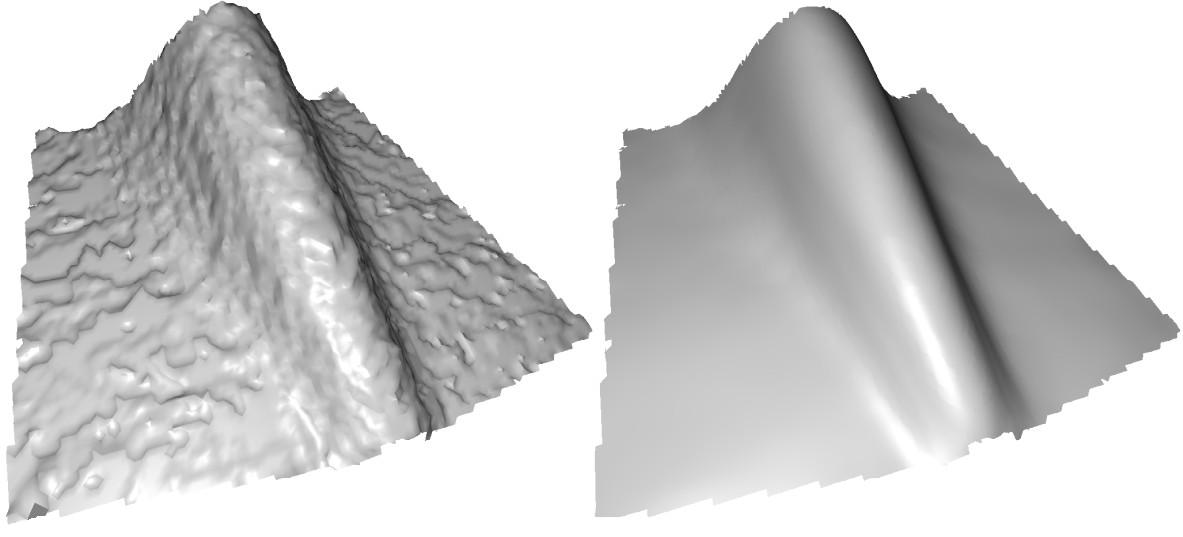
\includegraphics[scale=0.3]{dados/figuras/mls_filter.jpg}
    \caption{Exemplo do uso do Filtro de Suavização.}
    \vspace{-0.8em}
    \fonte{Adaptado de \cite{ridel2015mls}.}
    \label{fig:smoothing_filter}
\end{figure}

No trabalho, o filtro é utilizado com o intuito de suavizar e corrigir boa parte do ruído e pequenos erros de medição de distância gerado nos dados, provenientes da movimentação do robô enquanto realiza a coleta.

\section{Reconstrução}
\label{sec:reconstrucao}

A reconstrução do modelo tridimensional é gerada a partir da nuvem de pontos, onde é obtido a forma final da superfície. 
Como exemplo, a Figura \ref{fig:reconstruction} mostra a reconstrução de um objeto passo a passo.

\begin{figure}[H]
    \centering
    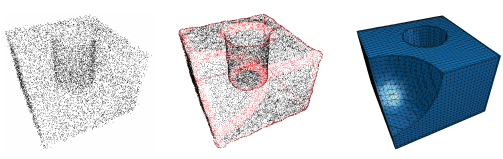
\includegraphics[scale=0.8]{dados/figuras/reconstruction.png}
    \caption{Reconstrução de um objeto em 3D a partir de uma nuvem de pontos.}
    \vspace{-0.8em}
    \fonte{Adaptado de \cite{jenke2006bayesian}.}
    \label{fig:reconstruction}
\end{figure}

Para dar forma à superfície é necessário uma lógica para ligar os pontos, tal lógica é conhecida como triangulação.
No trabalho, a triangulação é feita através da construção de triângulos sem fazer sobreposições. 
Apesar do nome triangulação remeter à triângulos, ela pode ser constituída por qualquer espaço em simplexos ou polígonos. 
Os simplexos são extensões de triângulos em outras dimensões, tais como segmentos de reta, tetraedros, triângulos e etc. 
Os elementos que constituem uma triangulação, são denominados de face.
A Figura \ref{fig:triangulation} mostra algumas formas para fazer a triangulação em um conjunto de pontos, como a triangulação incremental e a triangulação do fecho convexo.

\begin{figure}[H]
    \centering
    \begin{subfigure}[t]{0.9\textwidth}
        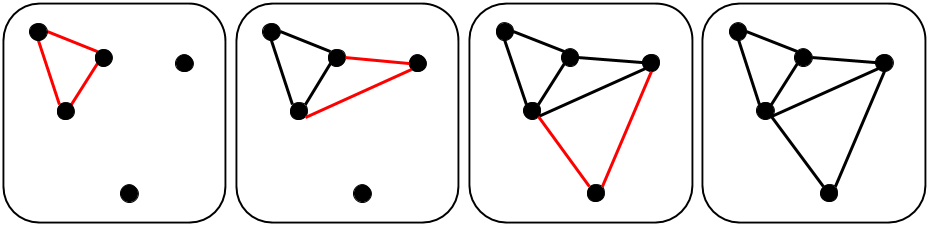
\includegraphics[width=\textwidth]{dados/figuras/triangulation_incremental.png}
        \caption{Triangulação Incremental}
        \label{fig:incremental_triangulation}
        \vspace{1em}
    \end{subfigure}
    \begin{subfigure}[t]{0.9\textwidth}
        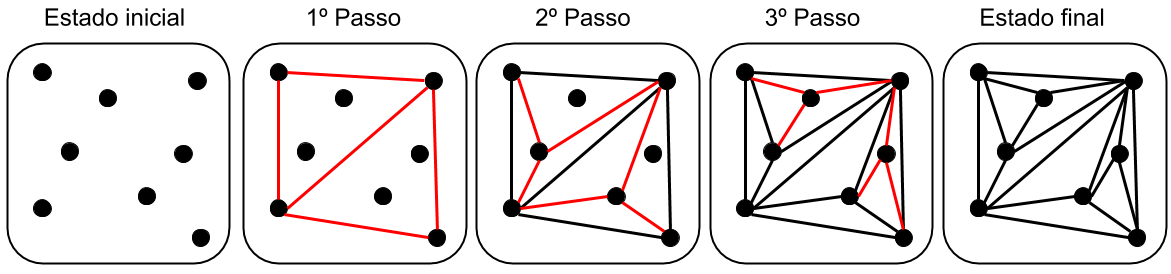
\includegraphics[width=\textwidth]{dados/figuras/triangulation_convex.png}
        \caption{Triangulação do Fecho Convexo}
        \label{fig:convex_triangulation}
    \end{subfigure}
    \caption{Exemplos de modelos de triangulação.}
    \label{fig:triangulation}
\end{figure}

Na Figura \ref{fig:incremental_triangulation} mostra a triangulação incremental, onde é realizada a construção de triângulos a partir da seleção aleatória do ponto inicial, seguindo a ligação pelo ponto mais próximo. 
Na Figura \ref{fig:convex_triangulation} mostra a triangulação do fecho convexo, na qual se realiza o fecho convexo do conjunto de pontos seguindo pela triangulação.
Após esse primeiro passo, para cada ponto no interior dos triângulos formados, se divide em mais três triângulos.

Fecho convexo (também conhecido como invólucro convexo ou envoltório convexo) é uma estrutura composta pelo subconjunto de pontos marginais de um conjunto de pontos. No plano, o fecho convexo é um polígono, enquanto que no espaço é representado por uma superfície fechada (Figura \ref{fig:convex_hull}).

\begin{figure}[H]
    \centering
    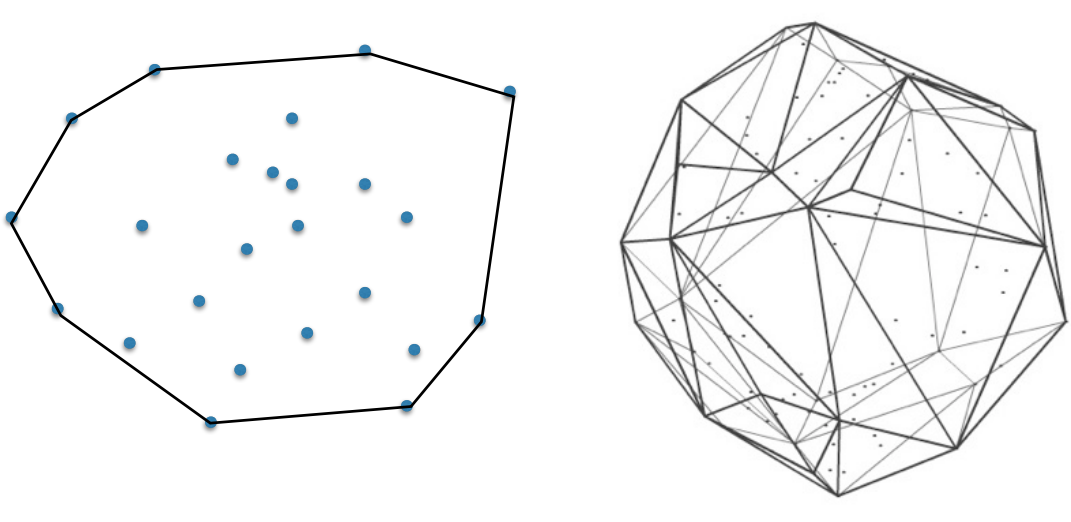
\includegraphics[scale=0.4]{dados/figuras/convex_hull.png}
    \caption{Fecho convexo representado no plano (esquerda) e no espaço (direita).}
    \label{fig:convex_hull}
\end{figure}

Uma triangulação nem sempre é adequada para um certo problema, pois os triângulos precisam ser semelhantes com o triângulo equilátero (triângulos que não possuem ângulos internos agudos). Essas triangulações especiais usam critérios detalhados a seguir para definir triângulos, entre os modelos conhecidos existe a Triangulação de Delaunay.


\subsection{Triangulação de Delaunay}
\label{sec:delaunay}
A triangulação de Delaunay, proposto por \cite{delaunay1934sphere}, é o método responsável por fornecer uma triangulação composta por triângulos semelhantes ao triângulo equilátero, em um determinado conjunto de pontos. O método pode ser formulado e estudado no espaço euclidiano de dimensão $n$, mas para fins didáticos será definida e exemplificada apenas no plano.
Para a criação dos triângulos, se pode utilizar qualquer metodologia de triangulação (inclusive as que foram apresentadas na Figura \ref{fig:triangulation}).

Após a criação, há uma verificação, que deve ser realizada em cada triângulo da malha, definida pela regra do circuncirculo, que determina se o triângulo é ou não de Delaunay. 
A regra descreve que para cada triângulo da malha, é traçado um círculo que passa pelos três vértices do triângulo, se esse círculo conter apenas os 3 pontos do triângulo, então ele satisfaz a regra. 
Se haver mais de 3 pontos dentro, então é aplicada a troca (\textit{flip}) entre arestas contidas no círculo.

Para explicar o termo \textit{flip}, observe a Figura \ref{fig:delaunay1}, onde o triângulo ABC não satisfaz a regra do circuncirculo, pois há outro vértice contido (D).
Para resolver esse problema se utiliza o \textit{flip} entre os triângulos ABC e ACD, que faz a troca da aresta AC pela aresta DB. 
Refazendo a regra do circuncirculo nos triângulos, é possível observar (Figura \ref{fig:delaunay2}) que ambos agora são triângulos de Delaunay.

\begin{figure}[H]
    \centering
    \begin{subfigure}[t]{0.3\textwidth}
        \caption{Triangulação que não satisfaz o critério de Delaunay.}
        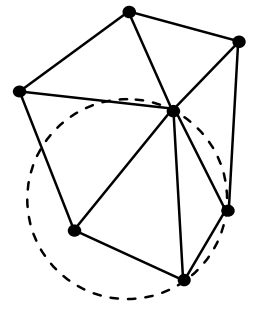
\includegraphics[width=\textwidth]{dados/figuras/delaunay1.png}
        \label{fig:delaunay1}
    \end{subfigure}
    \hspace{3em}
    \begin{subfigure}[t]{0.3\textwidth}
        \caption{Triangulação após o \textit{flip} entre arestas.}
        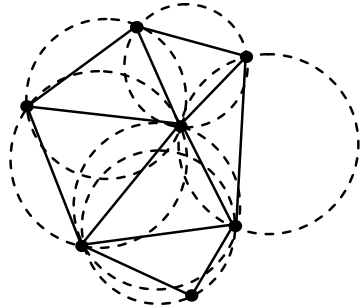
\includegraphics[width=\textwidth]{dados/figuras/delaunay2.png}
        \label{fig:delaunay2}
    \end{subfigure}
    \caption{Validação de triângulos utilizando a regra do circuncirculo e do \textit{flip}.}
    \vspace{-0.8em}
    \fonte{Adaptado de \cite{piteri2007triangulacao}.}
    \label{fig:delaunay}
\end{figure}

Na Figura \ref{fig:delaunay_theorem} há outro exemplo de \textit{flip}. A Figura \ref{fig:delaunay_theorem2} mostra ambos triângulos que não obedecem a regra do circuncírculo. Realizando o \textit{flip} entre as arestas BD e AC, a regra se torna válida (Figura \ref{fig:delaunay_theorem3}). 

\begin{figure}[H]
    \centering
    \begin{subfigure}[t]{0.2\textwidth}
        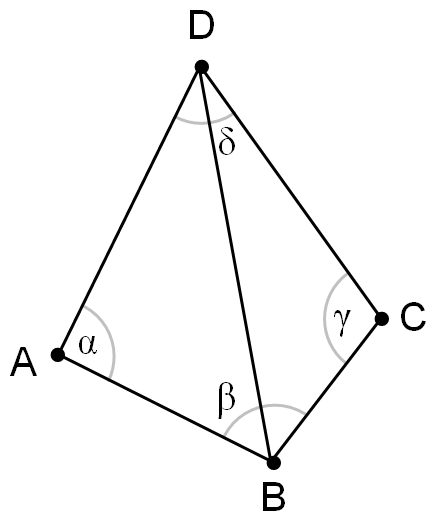
\includegraphics[width=\textwidth]{dados/figuras/delaunay_theorem1.png}
        \caption{}
        \label{fig:delaunay_theorem1}
    \end{subfigure}
    \hspace{2em}
    \begin{subfigure}[t]{0.27\textwidth}
        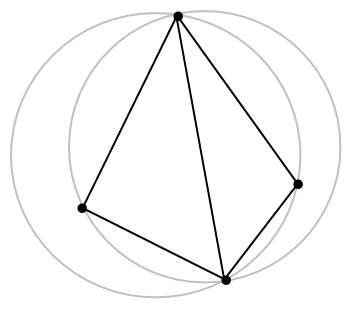
\includegraphics[width=\textwidth]{dados/figuras/delaunay_theorem2.png}
        \caption{}
        \label{fig:delaunay_theorem2}
    \end{subfigure}
    \hspace{2em}
    \begin{subfigure}[t]{0.2\textwidth}
        \includegraphics[width=\textwidth]{dados/figuras/delaunay_theorem3.png}
        \caption{}
        \label{fig:delaunay_theorem3}
    \end{subfigure}
    \caption{Regra do circuncírculo que define se um triângulo é ou não de Delaynay.}
    \label{fig:delaunay_theorem}
\end{figure}

Para realizar uma triangulação de um conjunto de pontos que estão dispersos pelo espaço é necessário projetá-los em um mesmo plano, pois só assim é possível reconstruir uma superfície aberta\footnote{Entende-se como superfície aberta qualquer forma ou geometria no espaço, no qual não possui volume, possui um ponto inicial e final e ambos pontos não se conectam, uma malha por exemplo. Uma superfície fechada possui um volume, que é o caso da esfera, do cubo, do toro etc.}.
Após a criação das faces, os pontos retornam para o espaço 3D.
Contudo, algumas faces podem conter pontos que estejam próximos no momento da triangulação no plano, mas distantes no espaço 3D, criando triângulos com uma grande área e que podem estar sobrepondo outros triângulos. 
Esse problema será tratado na próxima seção (Seção \ref{sec:split_mesh}).
Na Figura \ref{fig:prism} é possível observar uma projeção de pontos e faces em um plano.


\subsection{Separação da superfície}
\label{sec:split_mesh}

A separação da superfície é um processo que faz a divisão da malha e remove as sub-malhas desnecessárias, além de corrigir erros de reconstrução, utilizando a biblioteca Pymesh (descrita na Seção \ref{sec:pymesh}).
Essa etapa ocorre dentro da etapa de reconstrução, pois ela precisa atuar na malha já reconstruída e não na nuvem de pontos como ocorre na etapa de filtragem.

Como visto na seção anterior, a etapa de triangulação de uma nuvem de pontos no plano pode criar triângulos sobrepostos e com uma grande área (Figura \ref{fig:split_mesh2}).
Para resolver esse problema, é necessário definir um valor para a  área máxima do triângulo, ou seja, se a área do triângulo criado for maior que o valor definido de área máxima, então essa face é descartada da malha.
O valor definido para a área máxima pode depender do tamanho e da densidade da nuvem de pontos.
Essa abordagem resolve o problema, porém com o descarte de faces, acaba surgindo lacunas e descontinuidades na malha, gerando sub-malhas (Figura \ref{fig:split_mesh3}).

\begin{figure}[H]
    \centering
    \begin{subfigure}[t]{0.4\textwidth}
        \includegraphics[width=\textwidth]{dados/figuras/split_mesh1.png}
        \caption{Nuvem de pontos antes da reconstrução.}
        \label{fig:split_mesh1}
    \end{subfigure}
    \begin{subfigure}[t]{0.4\textwidth}
        \includegraphics[width=\textwidth]{dados/figuras/split_mesh2.png}
        \caption{Superfície sem aplicar a separação.}
        \label{fig:split_mesh2}
    \end{subfigure}
    \begin{subfigure}[t]{0.4\textwidth}
        \includegraphics[width=\textwidth]{dados/figuras/split_mesh3.png}
        \caption{Superfície após a remoção dos grandes triângulos.}
        \label{fig:split_mesh3}
    \end{subfigure}
    \begin{subfigure}[t]{0.4\textwidth}
        \includegraphics[width=\textwidth]{dados/figuras/split_mesh4.png}
        \caption{Superfície após a remoção das sub-malhas.}
        \label{fig:split_mesh4}
    \end{subfigure}
    \caption{Processo de remoção das sub-malhas.}
    \label{fig:split_mesh}
\end{figure}

Para escolher a sub-malha que represente melhor a superfície escaneada pelo sensor, se faz o cálculo de área de cada sub-malha.
Aquela que apresentar maior área será escolhida e o restante será descartado (Figura \ref{fig:split_mesh4}).


\section{Comparação}
\label{sec:comparacao}

A comparação é a última etapa da metodologia. 
Essa parte faz a comparação entre dois modelos e determinar o quanto se perdeu ou ganhou em relação ao volume e superfície. 
A principal aplicação é modelar coletas do mesmo local em diferentes períodos e fazer a comparação entre os resultados alcançados.

Os resultados são obtidos a partir da diferença entre dois modelos reconstruídos, por esse motivo a etapa de comparação é um processo separado do restante. 
O cálculo de superfície ocorre nas etapas de reconstrução e comparação, enquanto que o cálculo de volume só ocorre na etapa de comparação, por isso ambos serão descritos nesta seção.

\subsection{Cálculo de superfície}
\label{sec:surface_calc}

O cálculo da área de superfície é importante para estimar a qualidade da reconstrução.
A superfície é uma malha de triângulos, portanto para calcular a área total, basta somar a área de cada triângulo contido nela. 
Para esse tipo de cálculo foi utilizada a fórmula de Heron (ou de Herão), que é capaz de calcular a área de qualquer tipo de triângulo em função das medidas dos seus três lados.
A fórmula de Heron é mostrada pela Equação \ref{eq:heron}, onde $a$, $b$ e $c$ são os três lados e $p$ representa o semiperímetro do triângulo.

\begin{equation}
    A = \sqrt{p(p-a)(p-b)(p-c)}
    \label{eq:heron}
\end{equation}

\begin{equation}
    p = \frac{a+b+c}{2}
    \label{eq:heron_p}
\end{equation}


\subsection{Cálculo de volume}
\label{sec:volume_calc}

O processo de cálculo de volume é fundamental para realizar a comparação entre reconstruções.
O volume é formado a partir da projeção da superfície do modelo em um plano base, como mostra na Figura \ref{fig:prism}.
O resultado da projeção é um conjunto de poliedros irregulares, onde cada poliedro possui uma base inferior diferente da base superior.

\begin{figure}[H]
    \centering
    \includegraphics[scale=0.5]{dados/figuras/prisms.png}
    \caption{Formação do volume a partir da superfície.}
    \vspace{-0.8em}
    \fonte{\cite{berg2008computational}}
    \label{fig:prism}
\end{figure}

O plano base em uma comparação é definido pelo ponto coletado mais distante do sensor entre os dois modelos.
Com o ponto selecionado, o plano base é traçado e ambos modelos constroem seus volumes com base nesse plano.

Na Figura \ref{fig:projection_declined} é ilustrado o ROV coletando dados do cenário $C$ enquanto que na Figura \ref{fig:projection_wall3} mostra a coleta do cenário $A$.
Para não ficar tão repetitivo na explicação a seguir, o cenário $C$ e $A$ serão denominados de $CC$ e $CA$, respectivamente.

\begin{figure}[H]
    \centering
    \begin{subfigure}[t]{0.48\textwidth}
        \includegraphics[width=\textwidth]{dados/figuras/projection_wall3.jpg}
        \caption{}
        \label{fig:projection_wall3}
    \end{subfigure}
    \begin{subfigure}[t]{0.48\textwidth}
        \includegraphics[width=\textwidth]{dados/figuras/projection_declined.jpg}
        \caption{}
        \label{fig:projection_declined}
    \end{subfigure}
    \caption{ROV realizando a coleta de dados nos cenários $A$ (esquerda) e $C$ (direita).}
\end{figure}

Na comparação entre estes dois cenários, se nota que o ponto coletado que está mais distante do sensor pertence ao $CC$ (considerando apenas a parede dos ambientes).
A partir deste ponto mais distante se traça o plano base.
Com o plano base definido, o volume do $CC$ é gerado como mostra a Figura \ref{fig:projection1}.
Para ilustrar a diferença entre ambos cenários, a Figura \ref{fig:projection2} mostra a nuvem de pontos do $CA$ em comparação com o modelo reconstruído do $CC$.
Na Figura \ref{fig:projection3}, o $CA$ utiliza o mesmo plano base que foi usado no $CC$, para reconstruir o volume.
Após a reconstrução de ambos os volumes, se faz o cálculo do volume de cada modelo e, por fim, se compara os valores.

\begin{figure}[H]
    \centering
    \begin{subfigure}[t]{0.325\textwidth}
        \includegraphics[width=\textwidth]{dados/figuras/projection1.png}
        \caption{Volume que possui o ponto mais distante do sensor.}
        \label{fig:projection1}
    \end{subfigure}
    \begin{subfigure}[t]{0.325\textwidth}
        \includegraphics[width=\textwidth]{dados/figuras/projection2.png}
        \caption{Comparação entre a nuvem de pontos do $CA$ com o modelo do $CC$.}
        \label{fig:projection2}
    \end{subfigure}
    \begin{subfigure}[t]{0.325\textwidth}
        \includegraphics[width=\textwidth]{dados/figuras/projection3.png}
        \caption{Geração do volume do cenário $A$.}
        \label{fig:projection3}
    \end{subfigure}
    \caption{Reconstrução do volume de dois modelos em comparação.}
    \label{fig:projection}
\end{figure}

Como explicado no início da seção, a projeção da malha em um plano gera um volume que é composto por poliedros irregulares (Figura \ref{fig:prism}). O poliedro irregular é semelhante ao prisma regular, porém suas bases são diferentes (Figuras \ref{fig:polyhedron} e \ref{fig:regular_prisms}). Por essa razão, não se pode utilizar a fórmula do volume do prisma regular.  
Apesar de ser pouco provável, pode haver poliedros com a forma de um prisma regular.

\begin{figure}[H]
    \centering
    \begin{subfigure}[t]{0.3\textwidth}
        \includegraphics[width=\textwidth]{dados/figuras/pol_line.png}
        \caption{Poliedro em faces.}
        \label{fig:polyhedron1}
    \end{subfigure}
    \hspace{1em}
    \begin{subfigure}[t]{0.3\textwidth}
        \includegraphics[width=\textwidth]{dados/figuras/pol_solid.png}
        \caption{Poliedro em sólido.}
        \label{fig:polyhedron2}
    \end{subfigure}
    \hspace{1em}
    \begin{subfigure}[t]{0.3\textwidth}
        \includegraphics[width=\textwidth]{dados/figuras/pol_sep.png}
        \caption{Prisma e pirâmide destacados.}
        \label{fig:polyhedron3}
    \end{subfigure}
    \caption{Exemplo de um poliedro irregular.}
    \label{fig:polyhedron}
\end{figure}

\begin{figure}[H]
    \centering
    \includegraphics[scale=0.8]{dados/figuras/regular_prisms.jpg}
    \caption{Prismas regulares: são prismas que possuem ambas bases iguais.}
    \label{fig:regular_prisms}
\end{figure}

Antes de descrever o cálculo do volume, é importante saber que os dados utilizados como parâmetros são 6 pontos, sendo os 3 pontos da base inferior e os 3 pontos da base superior do poliedro irregular.
Para realizar esse cálculo, é necessário dividir o poliedro irregular na altura do ponto da base superior mais próximo à base inferior, representado pelo ponto $P$, como mostra a Figura \ref{fig:pol_sep3}.
O resultado da divisão é uma pirâmide irregular na parte superior e um prisma regular na parte inferior, como ilustra a Figura \ref{fig:polyhedron3}.

\begin{figure}[H]
    \centering
    \includegraphics[scale=0.7]{dados/figuras/pol_sep3.png}
    \caption{Base superior e inferior do poliedro irregular. O ponto $P$ representa o ponto da base superior que é mais próximo à base inferior.}
    \label{fig:pol_sep3}
\end{figure}

\begin{figure}[H]
    \centering
    \begin{subfigure}[t]{0.4\textwidth}
        \includegraphics[width=\textwidth]{dados/figuras/pyramid_line3.png}
        \caption{Pirâmide irregular. O ponto $a$ é o topo da pirâmide que está deitada.}
        \label{fig:pyramid_i}
    \end{subfigure}
    \hspace{2em}
    \begin{subfigure}[t]{0.4\textwidth}
        \includegraphics[width=\textwidth]{dados/figuras/prism_line2.png}
        \caption{Prisma regular.}
        \label{fig:prism_i}
    \end{subfigure}
    \caption{Poliedro separado em dois volumes.}
\end{figure}

A separação torna o cálculo do volume mais simples, como mostra a Equação \ref{eq:volume_polyhedron}. 
O volume total ($V_t$) é composto pela soma do volume da pirâmide ($V_{pi}$) com o volume do prisma ($V_{pr}$).
Na Equação \ref{eq:volume_pyramid}, o volume do prisma é $1/3$ do produto da base ($b_{pi}$) pela altura ($h_{pi}$). 
Por fim, o volume da pirâmide é o produto da base ($b_{pr}$) pela altura  ($h_{pr}$), como mostra a Equação \ref{eq:volume_prism}.
A área da base da pirâmide é um trapézio retângulo e é descrita pela Fórmula \ref{eq:trap_rect}, onde $B$ é a base maior ($\left | \overrightarrow{cb} \right |$)), $b$ é a base menor ($\left | \overrightarrow{de} \right |$)) e $h$ é a distância entre as bases ($\left | \overrightarrow{be} \right |$)


\begin{multicols}{3}
    \begin{equation}
        \label{eq:volume_polyhedron}
        V_t = V_{pr} + V_{pi}
    \end{equation}
    \begin{equation}
        \label{eq:volume_pyramid}
        V_{pr} = b_{pr} \cdot h_{pr}
    \end{equation}
    \begin{equation}
        \label{eq:volume_prism}
        V_{pi} = \frac{1}{3} \cdot b_{pi} \cdot h_{pi}
    \end{equation}
\end{multicols}

\begin{equation}
    \label{eq:trap_rect}
    b_{pi} = (B+b) \cdot h \cdot \frac{1}{2}
\end{equation}
\vspace{0.5em}

\iffalse
O Algoritmo \ref{alg:poly_alg} descreve o procedimento para o cálculo de volume de um poliedro irregular. 
O parâmetro de entrada são dois conjuntos de pontos que representam o triângulo da base inferior ($T_{inf}$) e o triângulo da base superior ($T_{sup}$).
Suponto que $p_a$ é o ponto mais próximo ao plano base, $p_b$ e $p_e$ são projeções dos pontos $p_c$, $p_d$ e $p_a$ (como ocorre no exemplo da Figura \ref{fig:pyramid_i}).

\vspace{1em}
\begin{algorithm}[H]
    \caption{Cálculo de Volume de um Poliedro Irregular}
    \hspace{1em}
    \KwIn{$T_{inf}$, $T_{sup}$}
    \KwOut{$V_t$}
    \For {$ponto \in T_{sup}$} {
        \If {$ponto$ for mais próximo ao plane base} {
            $p_a \leftarrow ponto$ \\
        }
    }
    $p_b \leftarrow$ proj($p_a$, $p_c$) \\
    $p_e \leftarrow$ proj($p_a$, $p_d$) \\
    
    $b_{pi} \leftarrow$ AreaBasePiramide($p_b$, $p_c$, $p_d$, $p_e$) \\
    $V_{pi} \leftarrow b_{pi} \cdot \left | proj(\overrightarrow{p_b p_a}, \overrightarrow{p_b p_e}) \right |$ \\
    $b_{pr} \leftarrow$ AreaBasePrisma($p_f$, $p_g$, $p_h$) \\
    $V_{pr} \leftarrow b_{pr} \cdot \left |\overrightarrow{p_a p_f} \right |$ \\
    $V_t \leftarrow V_{pi} + V_{pr}$ \\
    \label{alg:poly_alg}
    \hspace{1em}
\end{algorithm}
\fi                % Metodologia
% RESULTADOS-------------------------------------------------------------------

\chapter{ANÁLISE E DISCUSSÃO DOS RESULTADOS}
\label{chap:resultados}

\begin{figure}[H]
    \centering
    \caption{Imagem acústica do sonar gerada em um ambiente de simulação.}
    \label{fig:imagem_gpu_msis}
    \begin{subfigure}[t]{0.5\textwidth}
        \includegraphics[width=\textwidth]{dados/figuras/wall2.jpg}
        \caption{Simulação do cenário no Gazebo.}
    \end{subfigure}
    \begin{subfigure}[t]{0.42\textwidth}
        \includegraphics[width=\textwidth]{dados/figuras/heightmap_wall.png}
        \caption{Imagem acústica correspondente.}
    \end{subfigure}
\end{figure}                % Resultados
% CONCLUSÃO--------------------------------------------------------------------

\chapter{CONCLUSÃO}
\label{chap:conclusao}

\section{Trabalhos Futuros}
\label{sec:trabalhos_futuros}

\section{Considerações Finais}
\label{sec:consideracoes_finais}

Observa-se que nenhum resultado obteve 100\% na taxa de acerto, porque isso é praticamente uma utopia.                                 % Conclusão
%\chapter{CRONOGRAMA}
\label{chap:cronograma}

O cronograma do projeto é apresentado logo abaixo. As tarefas estão separadas em meses, por conta disso, elas possuem um \textit{X} nos meses em que serão trabalhadas. Em verde são as tarefas ou parte delas que já foram concluídas. Já em amarelo, está as tarefas que estão em andamento. Em vermelho, são as que ainda não foram iniciadas.

\begin{figure}[H]
    \centering
    \includegraphics[scale=0.8]{dados/figuras/cronograma.png}
\end{figure}                 % Cronograma

\postextual
% INSERE ELEMENTOS PÓS-TEXTUAIS
% REFERÊNCIAS------------------------------------------------------------------

% Carrega o arquivo "base-referencias.bib" e extrai automaticamente as referências citadas

\bibliography{./base-referencias}
\bibliographystyle{abntex2-alf} % Define o estilo ABNT para formatar a lista de referências
% OBSERVAÇÕES------------------------------------------------------------------
% Este arquivo não precisa ser alterado.
           			   % Referências
%% APÊNDICES--------------------------------------------------------------------
\iffalse
\begin{apendicesenv}
\partapendices

% Primeiro apêndice------------------------------------------------------------
\chapter{Nome do apêndice} % Edite para alterar o título deste apêndice
\label{chap:apendiceA}

Lembre-se que a diferença entre apêndice e anexo diz respeito à autoria do texto e/ou material ali colocado.

Caso o material ou texto suplementar ou complementar seja de sua autoria, então ele deverá ser colocado como um apêndice. Porém, caso a autoria seja de terceiros, então o material ou texto deverá ser colocado como anexo.

Caso seja conveniente, podem ser criados outros apêndices para o seu trabalho acadêmico. Basta recortar e colar este trecho neste mesmo documento. Lembre-se de alterar o "label"{} do apêndice.

Não é aconselhável colocar tudo que é complementar em um único apêndice. Organize os apêndices de modo que, em cada um deles, haja um único tipo de conteúdo. Isso facilita a leitura e compreensão para o leitor do trabalho.

% Novo apêndice----------------------------------------------------------------
\chapter{Nome do outro apêndice}
\label{chap:apendiceB}

conteúdo do novo apêndice

\end{apendicesenv}
\fi             			   % Apêndices
%% ANEXO------------------------------------------------------------------------
\begin{anexosenv}
\partanexos

\chapter{Especificação do ROV LBV300-5}
\label{chap:especificacao_rov}
\begin{figure}[H]
    \centering
    \includegraphics[scale=0.38]{dados/figuras/especificacao_rov.png}
\end{figure}

Informações retiradas do link: <http://www.teledynemarine.com/lbv300-5>

\chapter{Especificação do Sonar Tritech Micron Sonar}
\label{chap:especificacao_sonar}
\begin{figure}[H]
    \centering
    \includegraphics[scale=0.4]{dados/figuras/especificacao_sonar.png}
\end{figure}

Informações retiradas do link: <http://www.tritech.co.uk/media/products/small-rov-mechanical-sector-scanning-sonar-tritech-micron.pdf?id=e3070c7b>

\end{anexosenv}
               			   % Anexos

\end{document}
